\chapter{Additional Results}
% TODO : WHEN SIM FINISHES, CONVERT ALL 2s TO 3s
% KEYWORDS: seed_3 --> seed_3 , random seed: 3 --> random seed: 3 , _s3 --> _s3
\section{High Spatial Autocorrelation Results}
The methods will be compared on target fields generated with an autocorrelation factor, $\sigma_{field}$, equal to the field width.

\clearpage
\subsection{$10\%$ Maximum Field Scan}
\begin{figure}[htb!]
    \centering
    \begin{subfigure}[t]{0.65\textwidth}
        \centering
        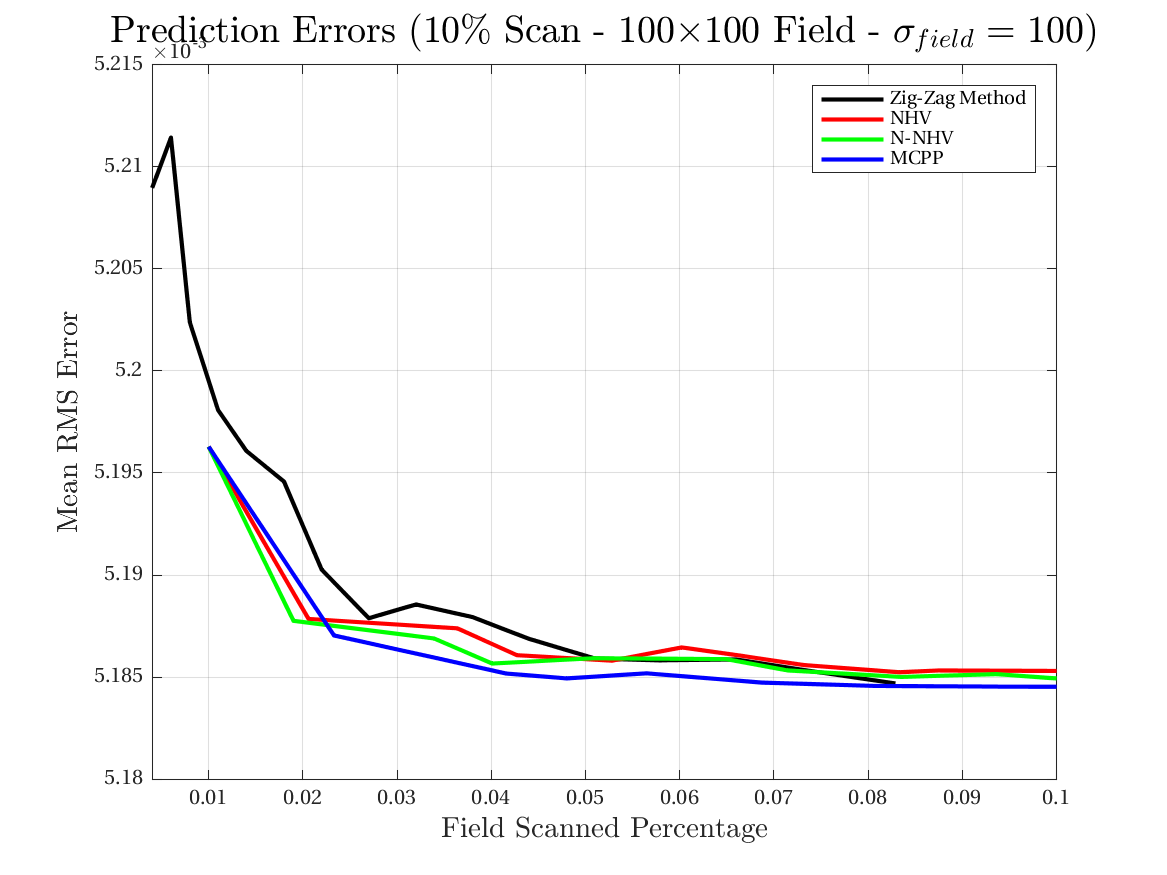
\includegraphics[width=\linewidth]{figures/hbresults/pred_errs_10p_100x100_sf_100_seed_3.png}
        \captionsetup{skip=0.20\baselineskip,size=footnotesize}
        \caption{Prediction errors (erf$(Z,\hat{Z})$).}
        \label{fig:prederrs_sigma100_p10_s3}
    \end{subfigure}%
    \\
    \begin{subfigure}[t]{0.65\textwidth}
        \centering
        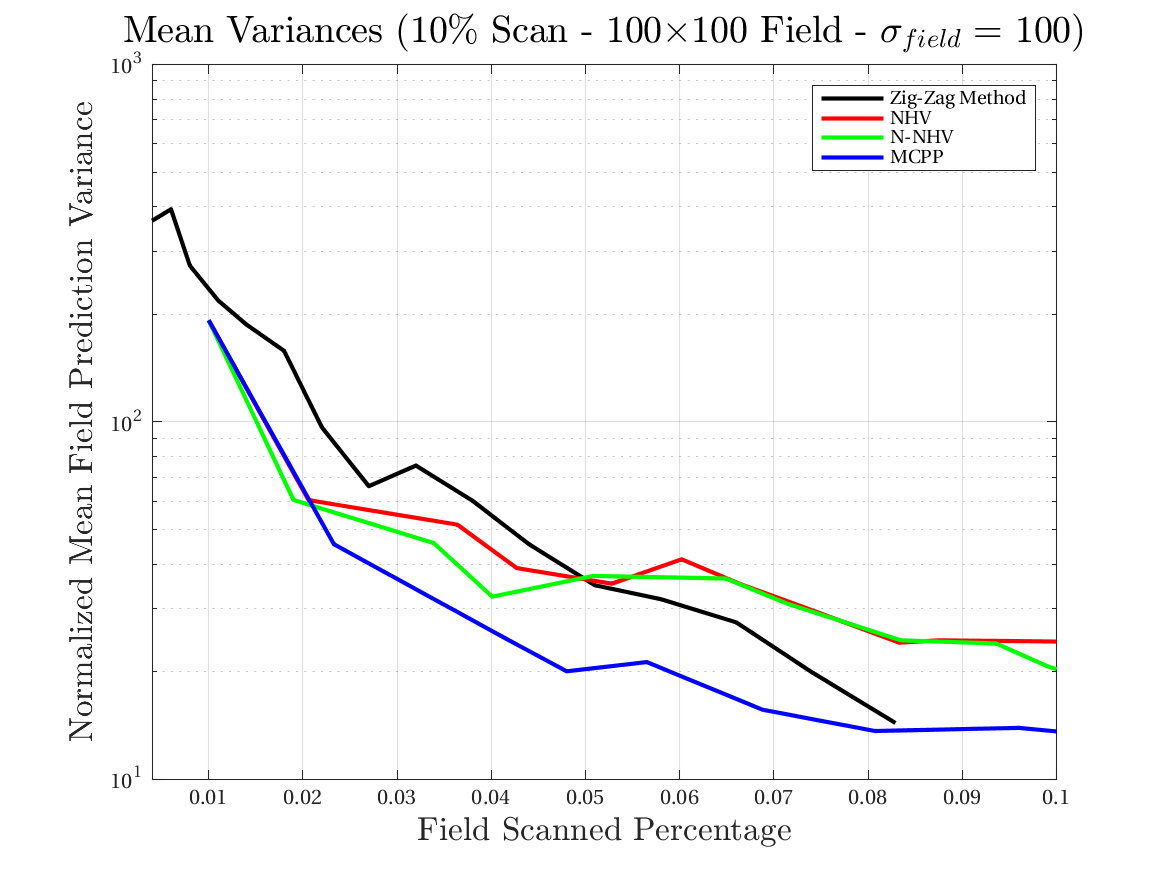
\includegraphics[width=\linewidth]{figures/hbresults/vars_10p_100x100_sf_100_seed_3.png}
        \captionsetup{skip=0.20\baselineskip,size=footnotesize}
        \caption{Semi-logarithmic prediction variances normalized to an a priori mean variance for the field.}
        \label{fig:prederrs_sigma100_p10_s3}
    \end{subfigure}
    \captionsetup{skip=0.20\baselineskip}
    \caption{A $10\%$ maximum area scan on a field of size $100 \times 100$, $\sigma_{field} = 100$, random seed: 3.}
    \label{fig:sigma100_p10_s3}
\end{figure}

\begin{figure}[htb!]
    \centering
    \begin{subfigure}[t]{0.5\textwidth}
        \centering
        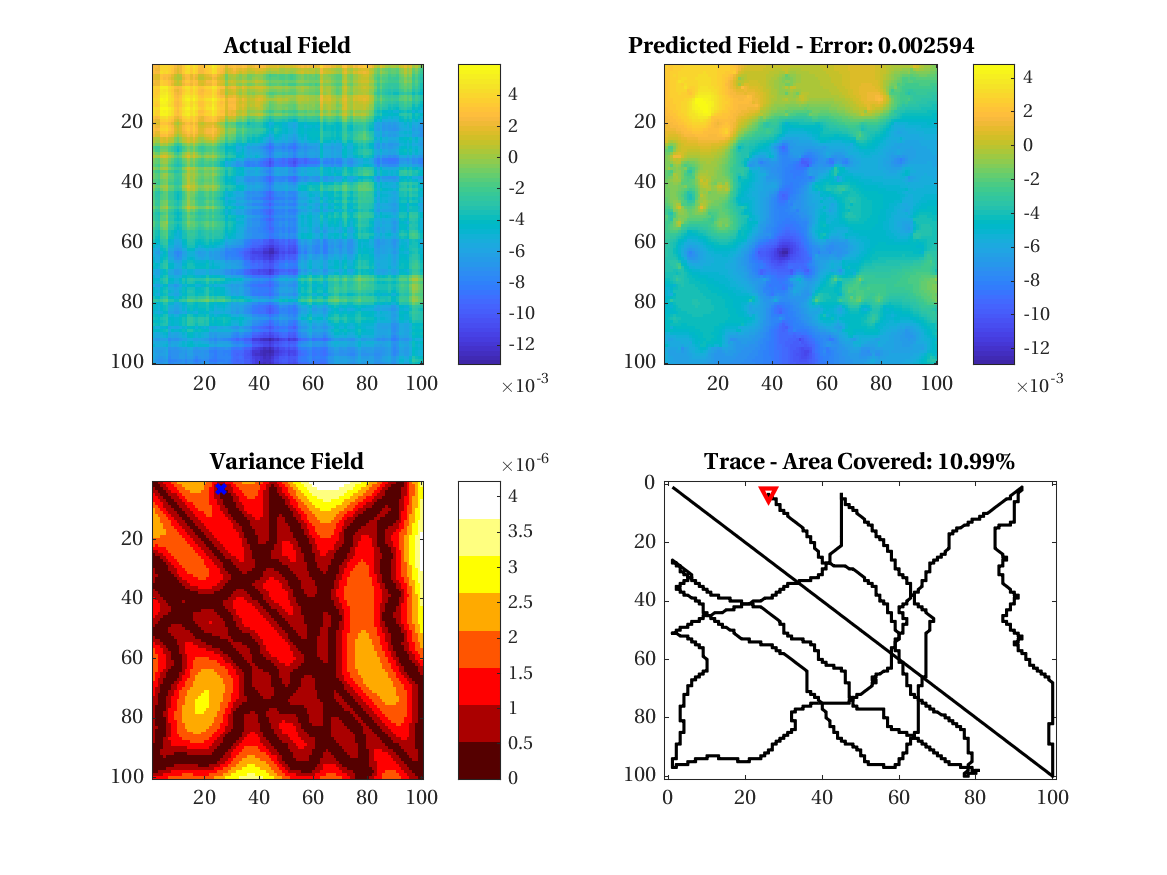
\includegraphics[width=\linewidth]{figures/hbresults/mc_10p_100x100_sf_100_seed_3.png}
        \captionsetup{skip=0.10\baselineskip,size=footnotesize}
        \caption{Monte Carlo Path Planner}
    \end{subfigure}%
    ~ 
    \begin{subfigure}[t]{0.5\textwidth}
        \centering
        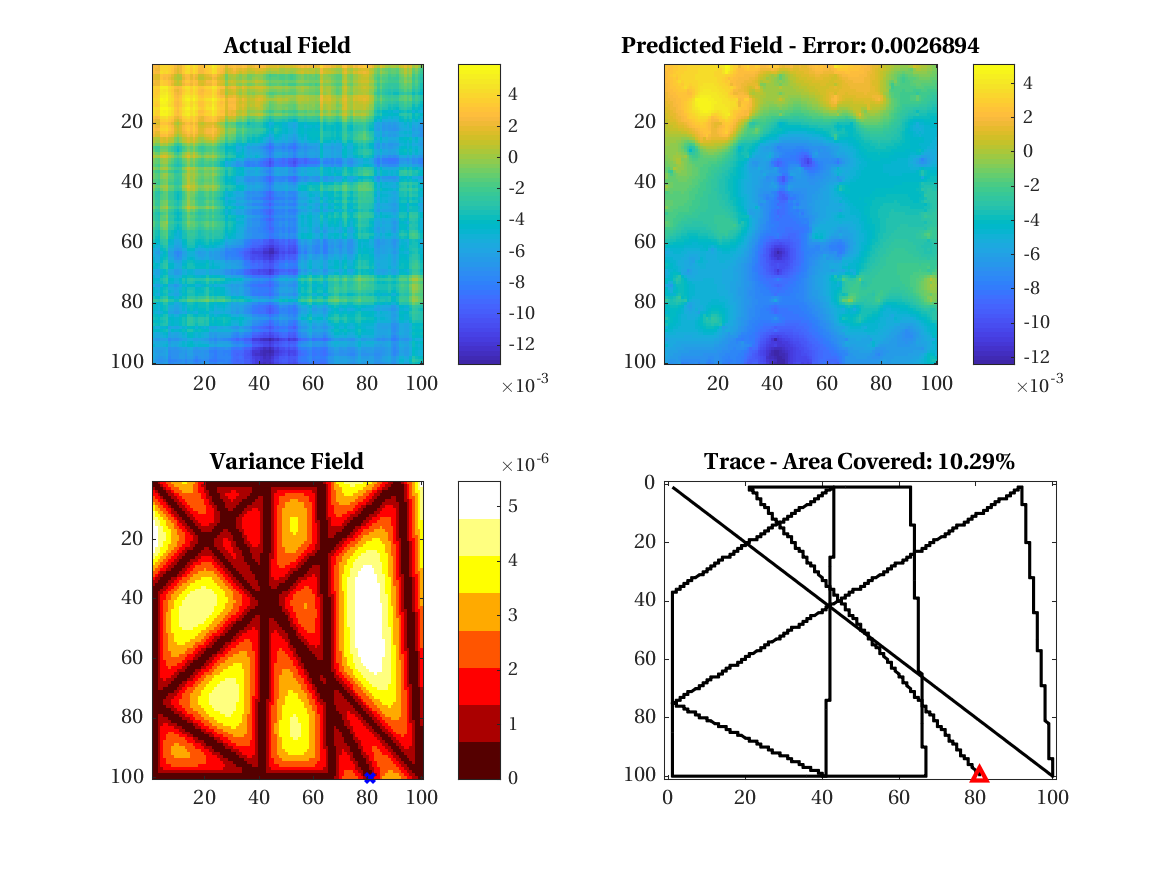
\includegraphics[width=\linewidth]{figures/hbresults/nhv_10p_100x100_sf_100_seed_3.png}
        \captionsetup{skip=0.10\baselineskip,size=footnotesize}
        \caption{Next Highest Variance Path Planner}
    \end{subfigure}%
    \\
    \begin{subfigure}[t]{0.5\textwidth}
        \centering
        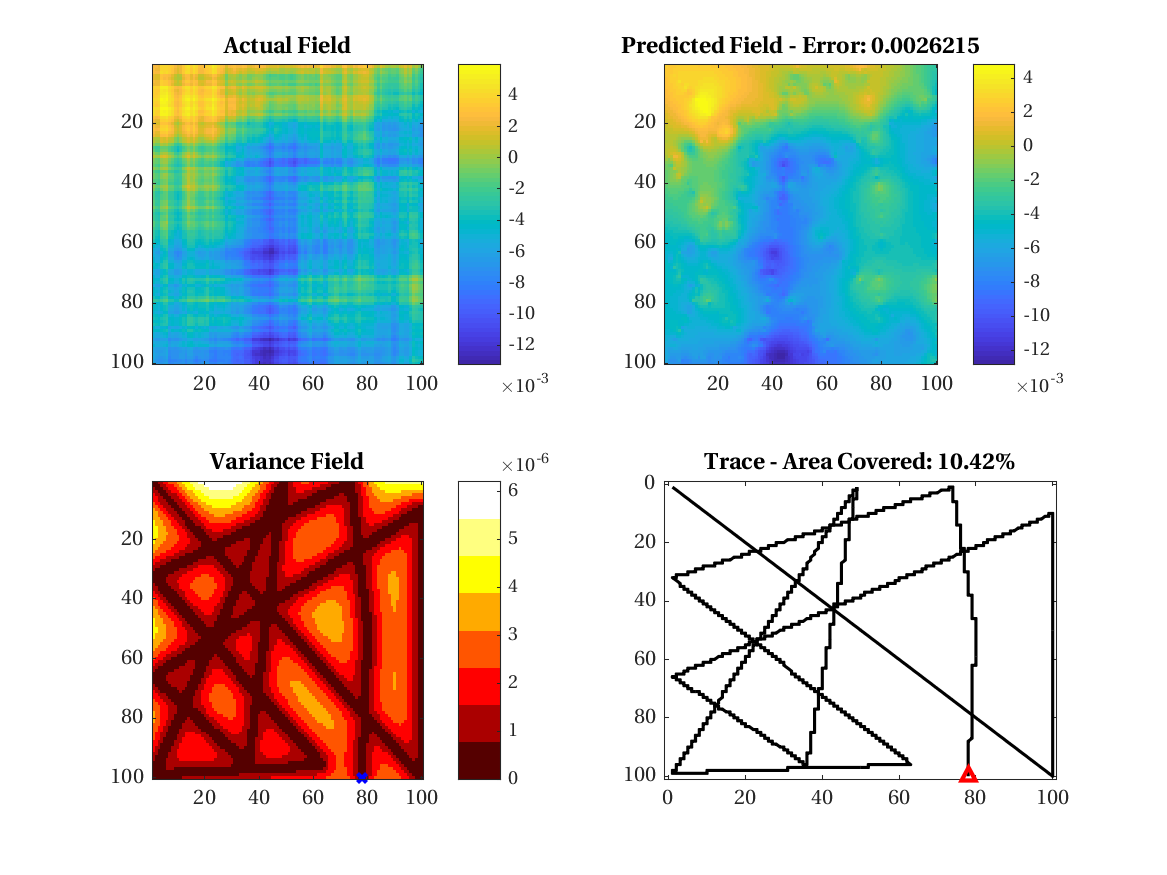
\includegraphics[width=\linewidth]{figures/hbresults/nnhv_10p_100x100_sf_100_seed_3.png}
        \captionsetup{skip=0.10\baselineskip,size=footnotesize}
        \caption{$N$ Next Highest Variance Path Planner}
    \end{subfigure}%
    ~
    \begin{subfigure}[t]{0.5\textwidth}
        \centering
        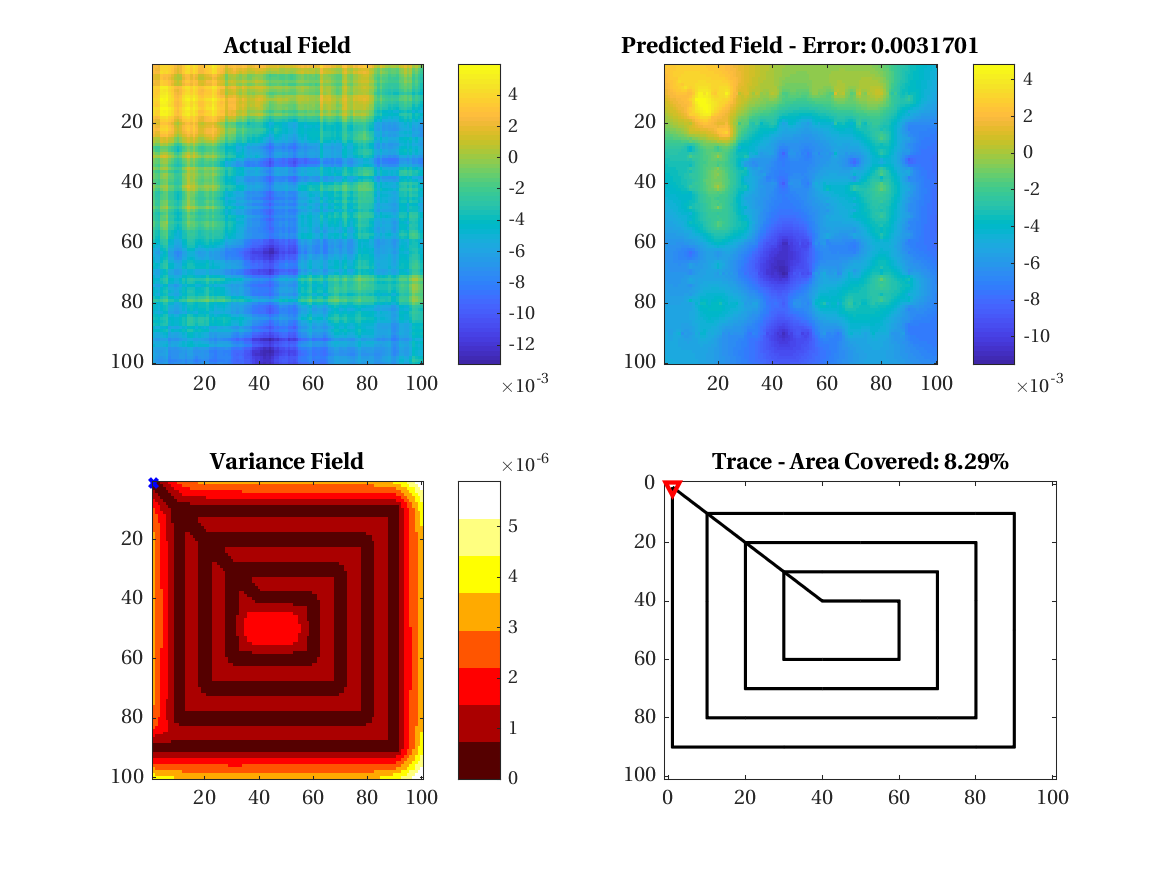
\includegraphics[width=\linewidth]{figures/hbresults/zz_10p_100x100_sf_100_seed_3.png}
        \captionsetup{skip=0.10\baselineskip,size=footnotesize}
        \caption{Zig-Zag Method}
    \end{subfigure}%
    \captionsetup{skip=0.20\baselineskip}
    \caption{Simulation output for a $10\%$ maximum area scan on a field of size $100 \times 100$, $\sigma_{field} = 100$, random seed: 3.}
    \label{fig:sim_sigma100_p10_s3}
\end{figure}

\FloatBarrier
\clearpage
\subsection{$20\%$ Maximum Field Scan}
\begin{figure}[htb!]
    \centering
    \begin{subfigure}[t]{0.65\textwidth}
        \centering
        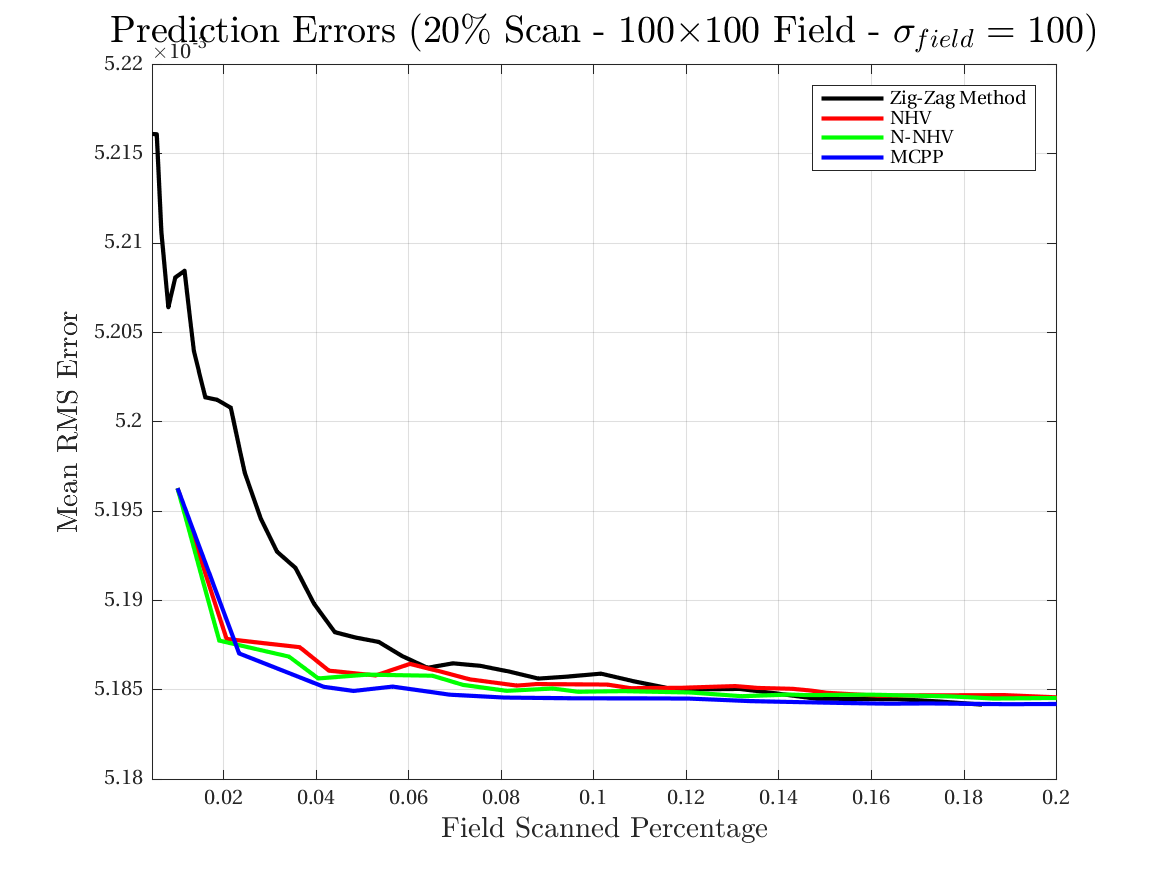
\includegraphics[width=\linewidth]{figures/hbresults/pred_errs_20p_100x100_sf_100_seed_3.png}
        \captionsetup{skip=0.20\baselineskip,size=footnotesize}
        \caption{Prediction errors (erf$(Z,\hat{Z})$).}
        \label{fig:prederrs_sigma100_p20_s3}
    \end{subfigure}%
    \\
    \begin{subfigure}[t]{0.65\textwidth}
        \centering
        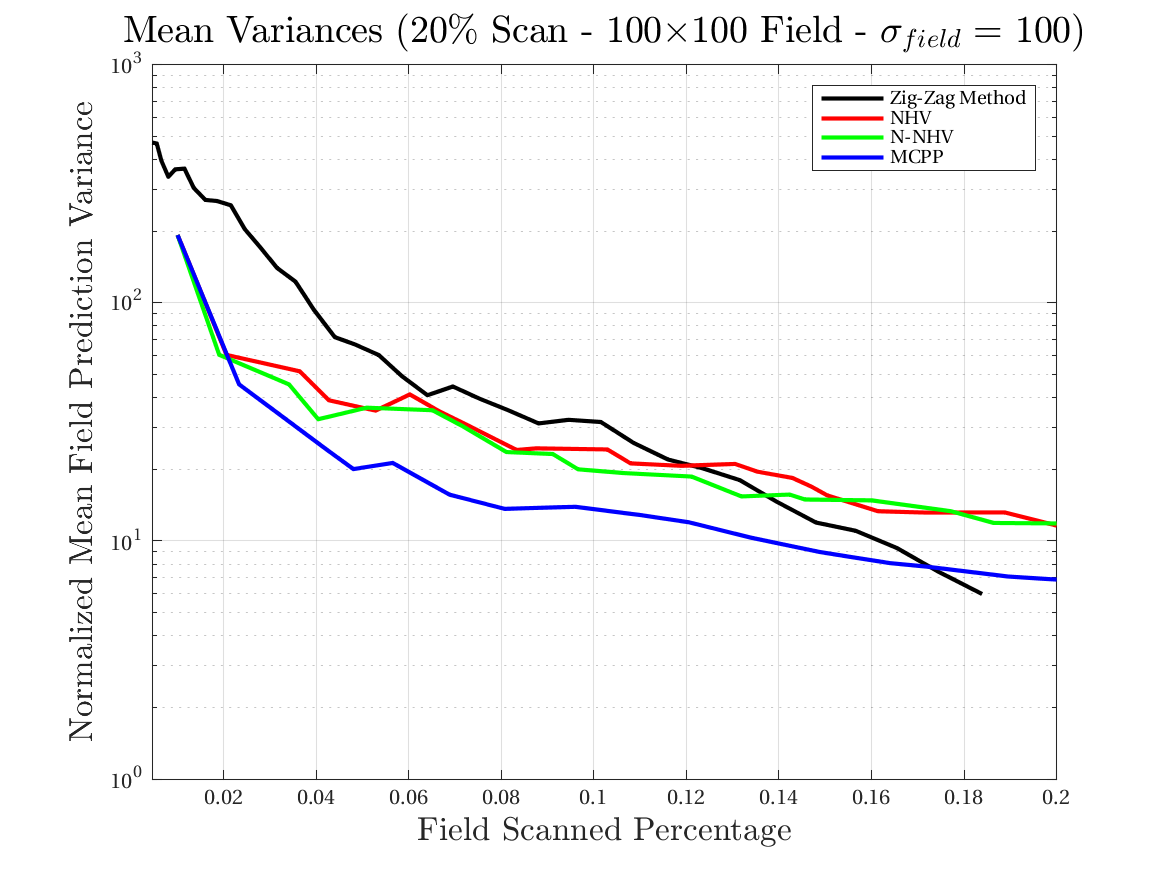
\includegraphics[width=\linewidth]{figures/hbresults/vars_20p_100x100_sf_100_seed_3.png}
        \captionsetup{skip=0.20\baselineskip,size=footnotesize}
        \caption{Semi-logarithmic prediction variances normalized to an a priori mean variance for the field.}
        \label{fig:prederrs_sigma100_p20_s3}
    \end{subfigure}
    \captionsetup{skip=0.20\baselineskip}
    \caption{A $20\%$ maximum area scan on a field of size $100 \times 100$, $\sigma_{field} = 100$, random seed: 3.}
    \label{fig:sigma100_p20_s3}
\end{figure}

\begin{figure}[htb!]
    \centering
    \begin{subfigure}[t]{0.5\textwidth}
        \centering
        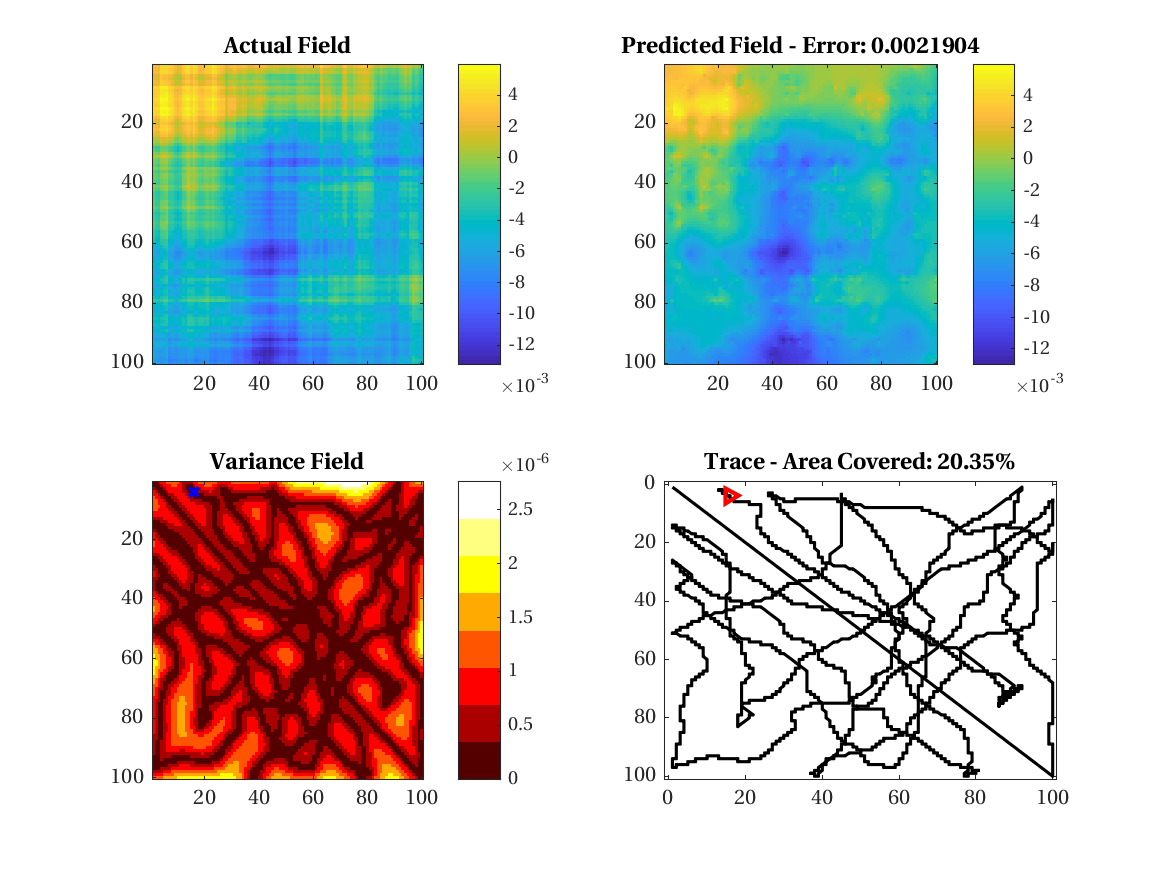
\includegraphics[width=\linewidth]{figures/hbresults/mc_20p_100x100_sf_100_seed_3.png}
        \captionsetup{skip=0.10\baselineskip,size=footnotesize}
        \caption{Monte Carlo Path Planner}
    \end{subfigure}%
    ~ 
    \begin{subfigure}[t]{0.5\textwidth}
        \centering
        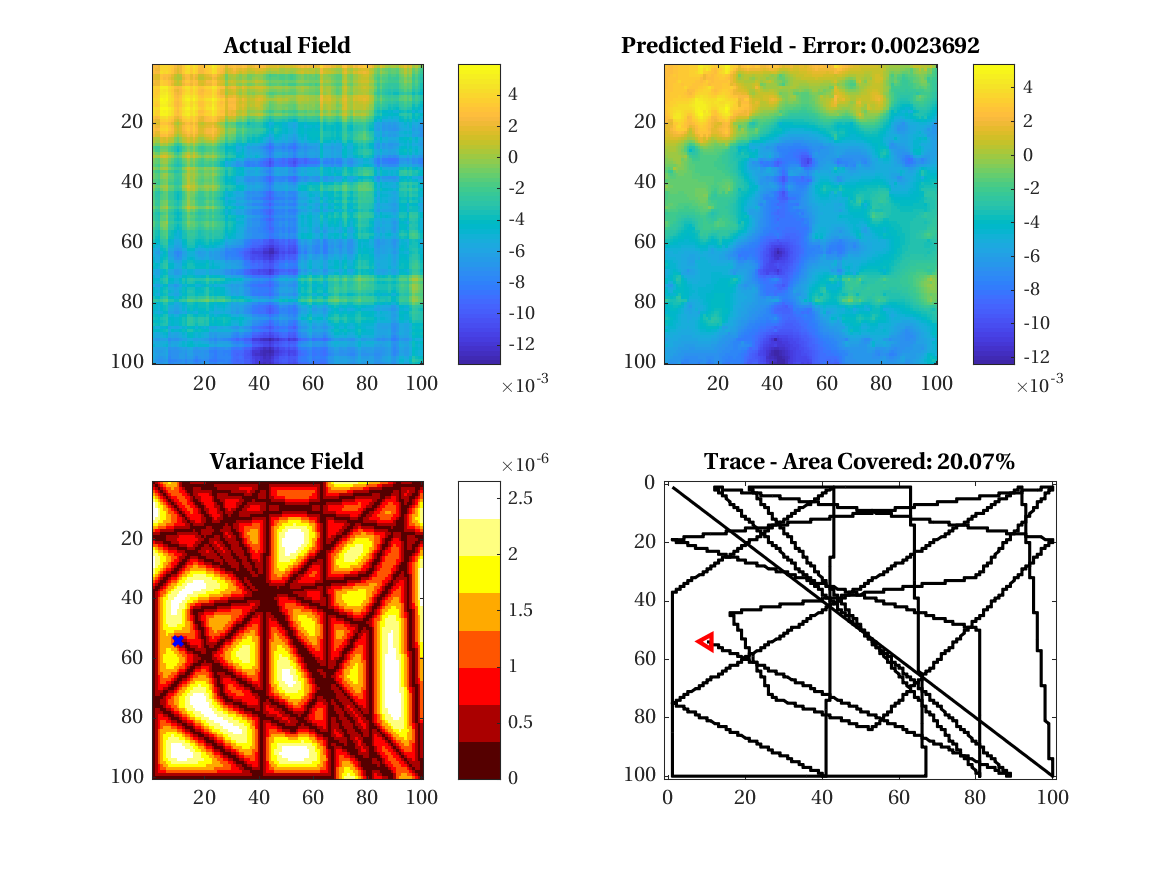
\includegraphics[width=\linewidth]{figures/hbresults/nhv_20p_100x100_sf_100_seed_3.png}
        \captionsetup{skip=0.10\baselineskip,size=footnotesize}
        \caption{Next Highest Variance Path Planner}
    \end{subfigure}%
    \\
    \begin{subfigure}[t]{0.5\textwidth}
        \centering
        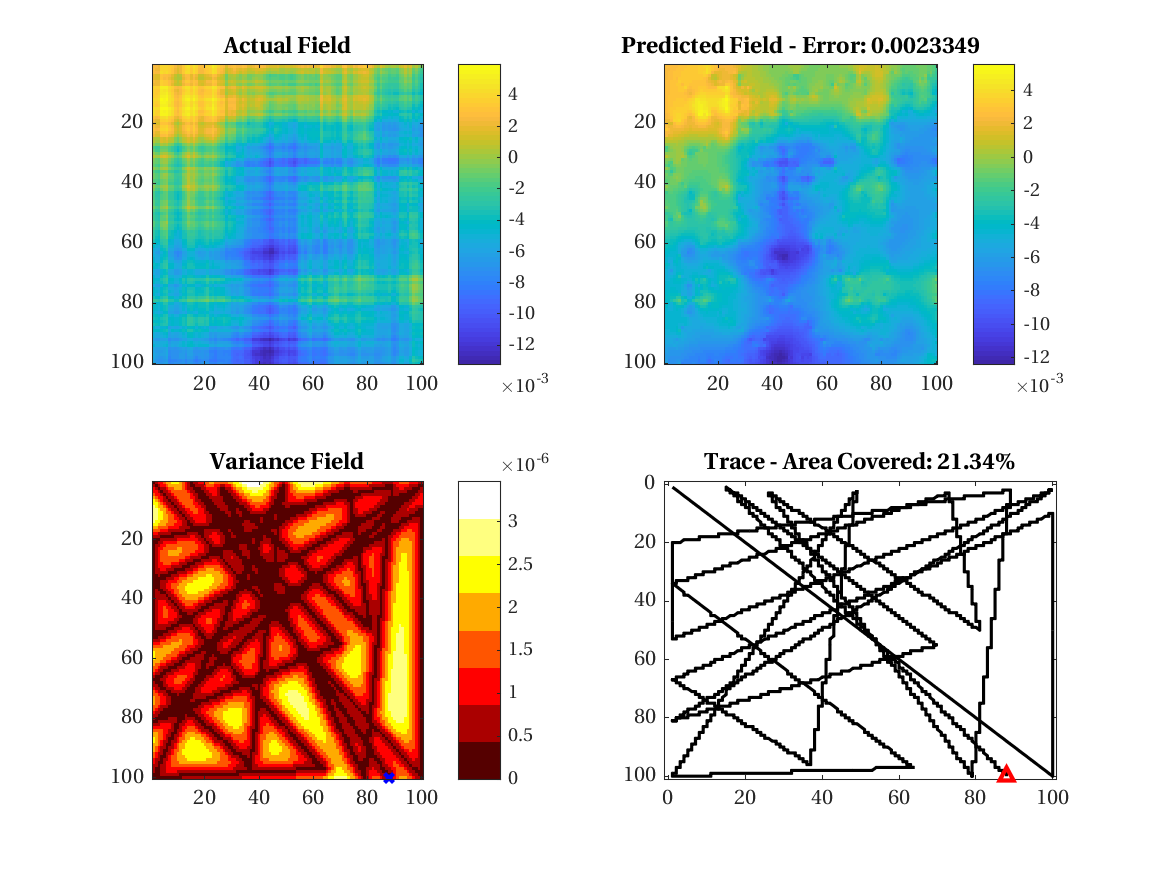
\includegraphics[width=\linewidth]{figures/hbresults/nnhv_20p_100x100_sf_100_seed_3.png}
        \captionsetup{skip=0.10\baselineskip,size=footnotesize}
        \caption{$N$ Next Highest Variance Path Planner}
    \end{subfigure}%
    ~
    \begin{subfigure}[t]{0.5\textwidth}
        \centering
        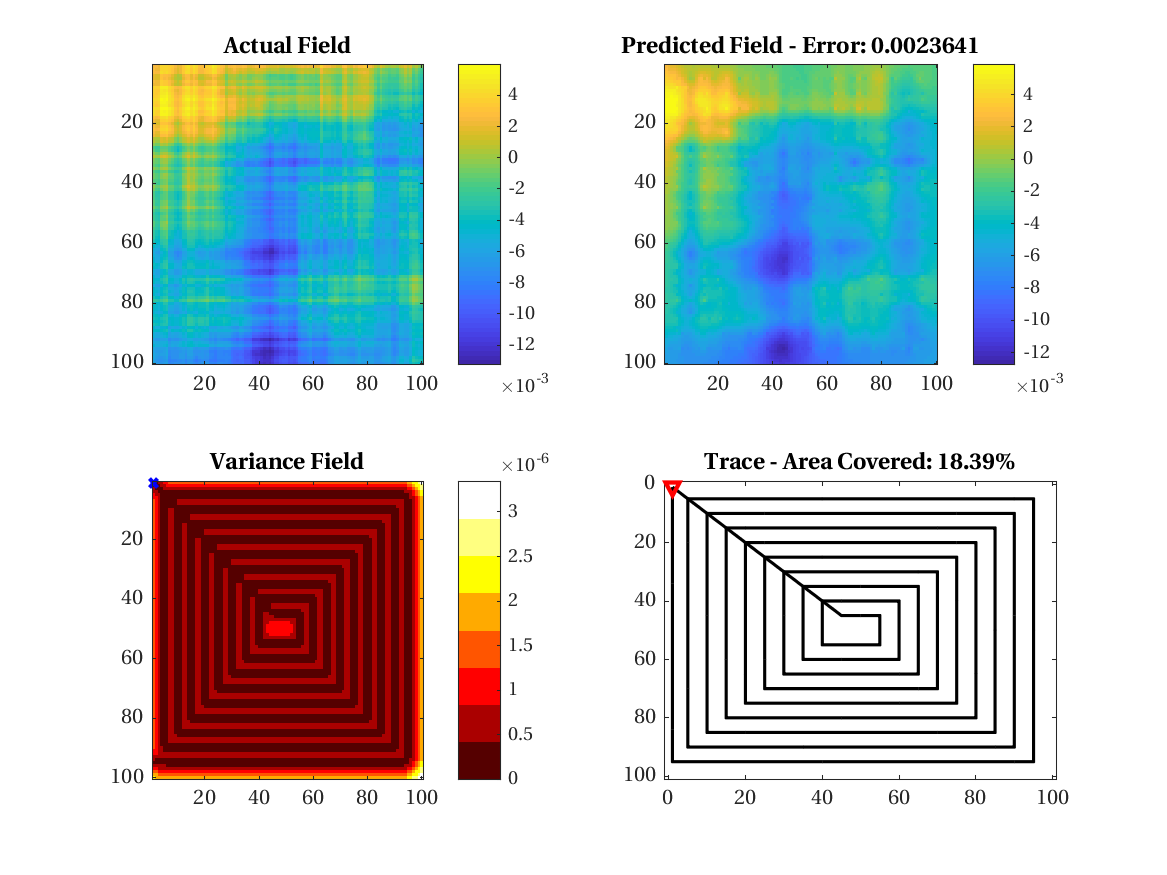
\includegraphics[width=\linewidth]{figures/hbresults/zz_20p_100x100_sf_100_seed_3.png}
        \captionsetup{skip=0.10\baselineskip,size=footnotesize}
        \caption{Zig-Zag Method}
    \end{subfigure}%
    \captionsetup{skip=0.20\baselineskip}
    \caption{Simulation output for a $20\%$ maximum area scan on a field of size $100 \times 100$, $\sigma_{field} = 100$, random seed: 3.}
    \label{fig:sim_sigma100_p20_s3}
\end{figure}

\FloatBarrier
\clearpage
\subsection{$30\%$ Maximum Field Scan}
\begin{figure}[htb!]
    \centering
    \begin{subfigure}[t]{0.65\textwidth}
        \centering
        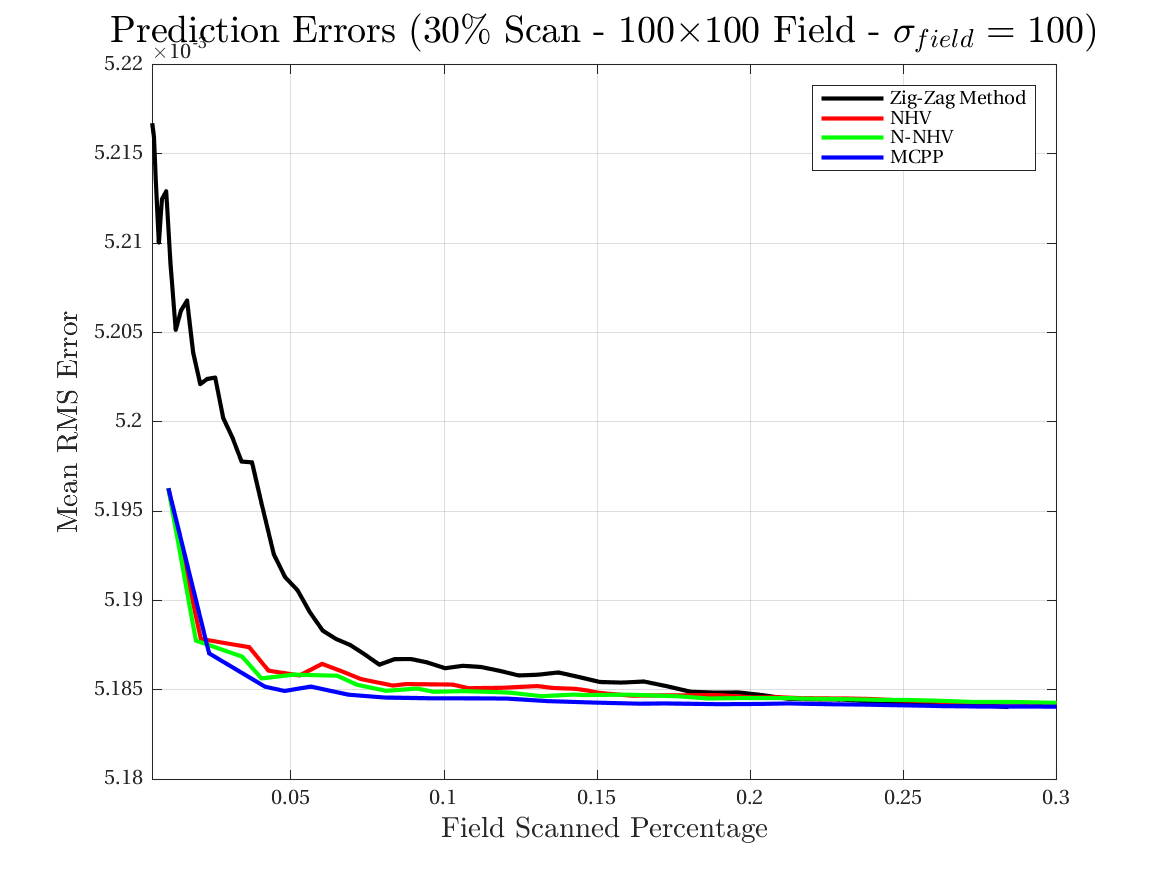
\includegraphics[width=\linewidth]{figures/hbresults/pred_errs_30p_100x100_sf_100_seed_3.png}
        \captionsetup{skip=0.20\baselineskip,size=footnotesize}
        \caption{Prediction errors (erf$(Z,\hat{Z})$).}
        \label{fig:prederrs_sigma100_p30_s3}
    \end{subfigure}%
    \\
    \begin{subfigure}[t]{0.65\textwidth}
        \centering
        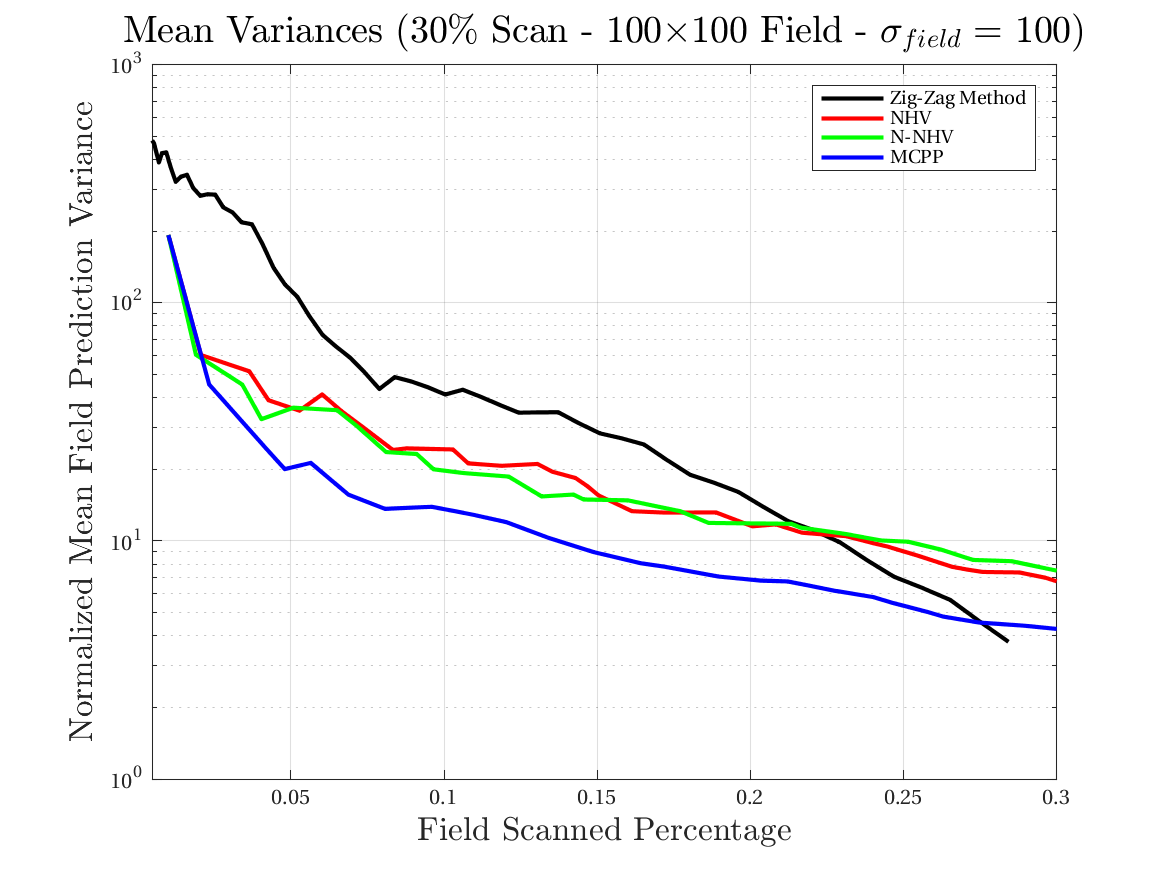
\includegraphics[width=\linewidth]{figures/hbresults/vars_30p_100x100_sf_100_seed_3.png}
        \captionsetup{skip=0.20\baselineskip,size=footnotesize}
        \caption{Semi-logarithmic prediction variances normalized to an a priori mean variance for the field.}
        \label{fig:prederrs_sigma100_p30_s3}
    \end{subfigure}
    \captionsetup{skip=0.20\baselineskip}
    \caption{A $30\%$ maximum area scan on a field of size $100 \times 100$, $\sigma_{field} = 100$, random seed: 3.}
    \label{fig:sigma100_p30_s3}
\end{figure}

\begin{figure}[htb!]
    \centering
    \begin{subfigure}[t]{0.5\textwidth}
        \centering
        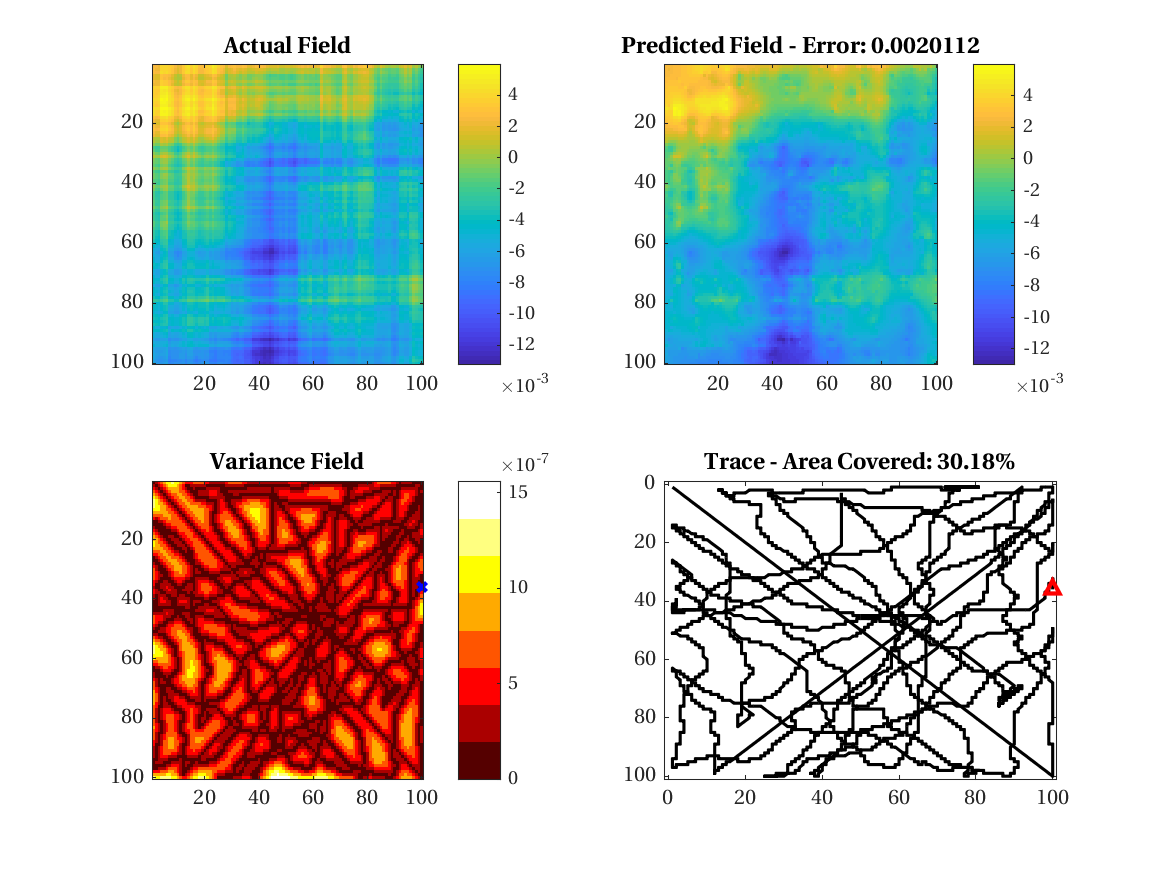
\includegraphics[width=\linewidth]{figures/hbresults/mc_30p_100x100_sf_100_seed_3.png}
        \captionsetup{skip=0.10\baselineskip,size=footnotesize}
        \caption{Monte Carlo Path Planner}
    \end{subfigure}%
    ~ 
    \begin{subfigure}[t]{0.5\textwidth}
        \centering
        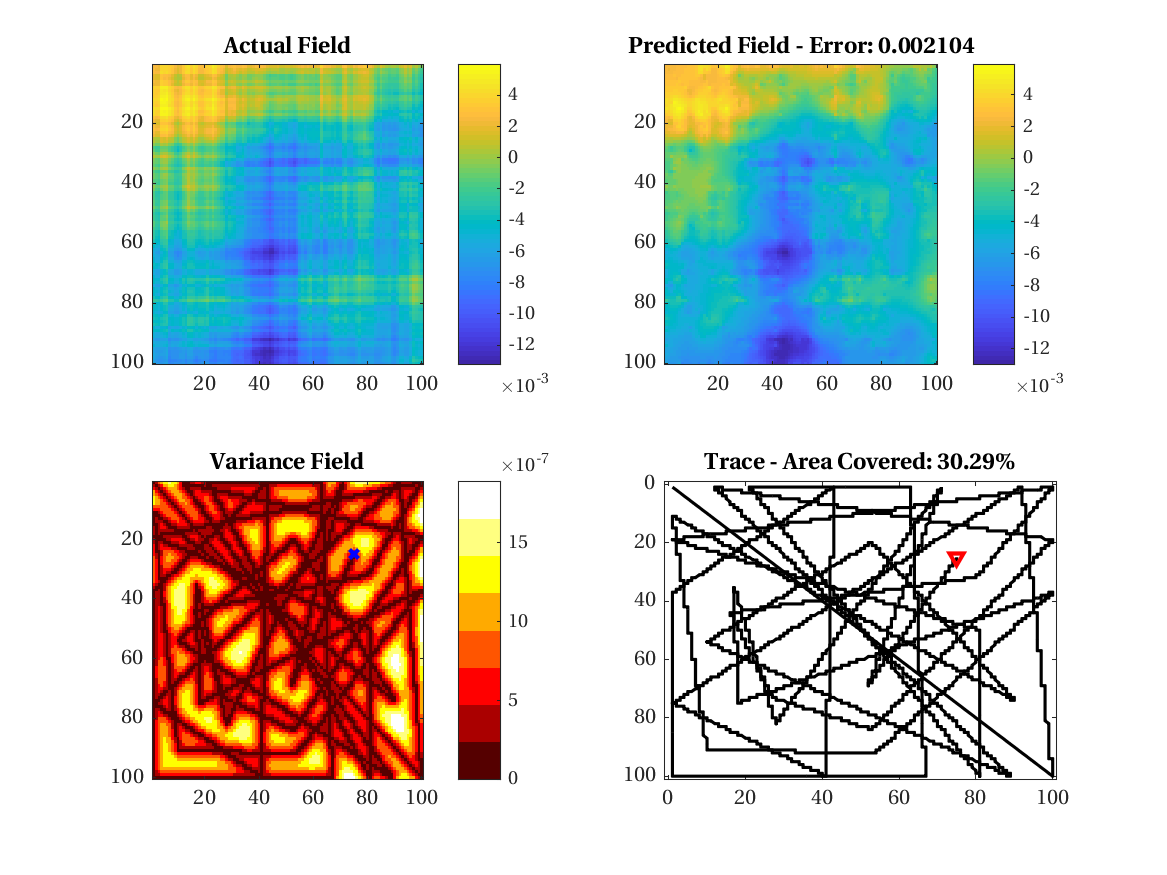
\includegraphics[width=\linewidth]{figures/hbresults/nhv_30p_100x100_sf_100_seed_3.png}
        \captionsetup{skip=0.10\baselineskip,size=footnotesize}
        \caption{Next Highest Variance Path Planner}
    \end{subfigure}%
    \\
    \begin{subfigure}[t]{0.5\textwidth}
        \centering
        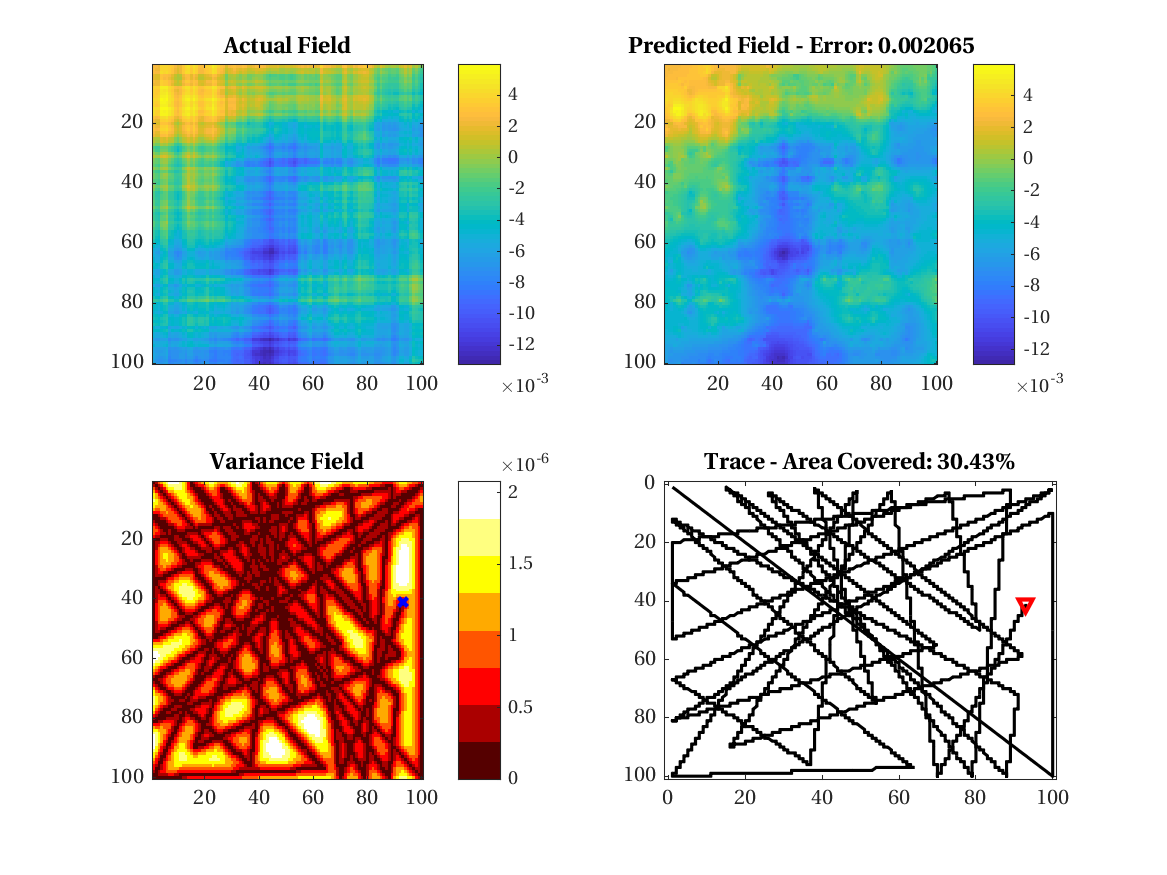
\includegraphics[width=\linewidth]{figures/hbresults/nnhv_30p_100x100_sf_100_seed_3.png}
        \captionsetup{skip=0.10\baselineskip,size=footnotesize}
        \caption{$N$ Next Highest Variance Path Planner}
    \end{subfigure}%
    ~
    \begin{subfigure}[t]{0.5\textwidth}
        \centering
        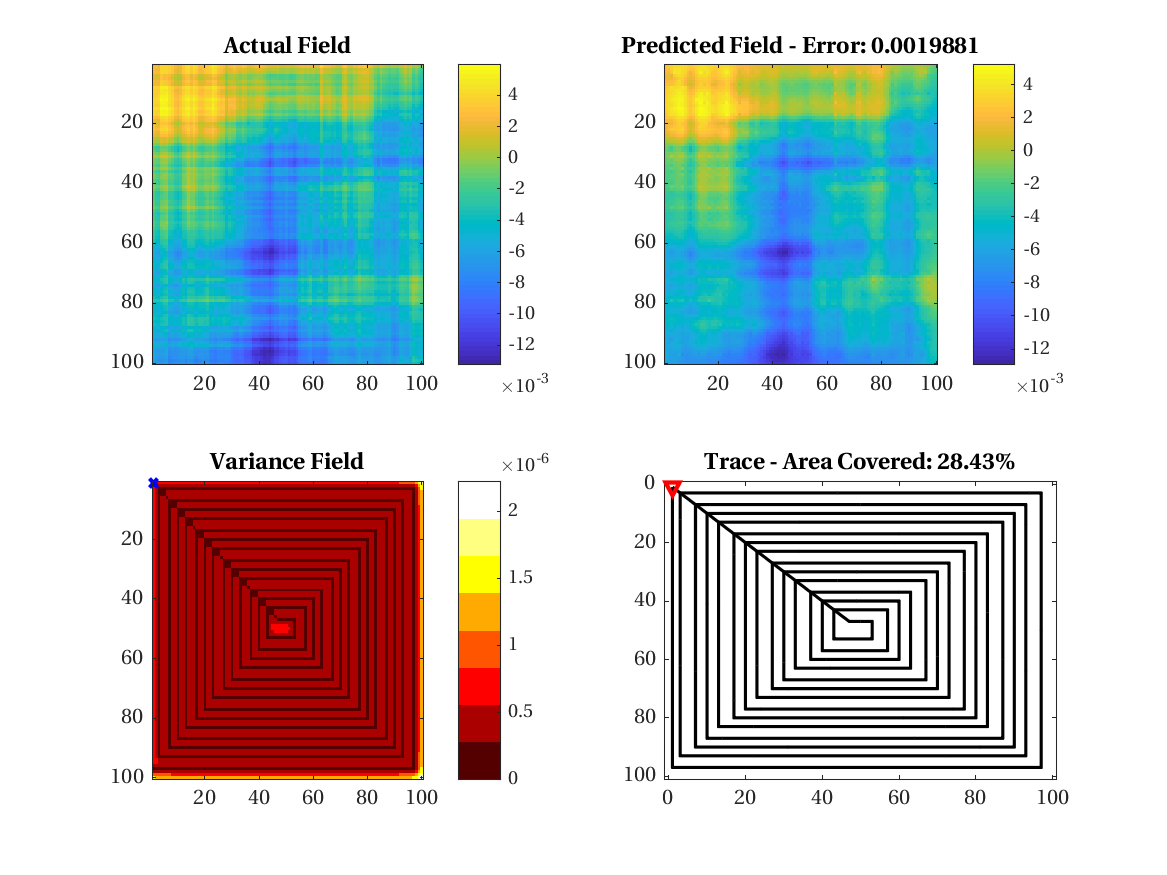
\includegraphics[width=\linewidth]{figures/hbresults/zz_30p_100x100_sf_100_seed_3.png}
        \captionsetup{skip=0.10\baselineskip,size=footnotesize}
        \caption{Zig-Zag Method}
    \end{subfigure}%
    \captionsetup{skip=0.20\baselineskip}
    \caption{Simulation output for a $30\%$ maximum area scan on a field of size $100 \times 100$, $\sigma_{field} = 100$, random seed: 3.}
    \label{fig:sim_sigma100_p30_s3}
\end{figure}
%% SIGMA HALF

\section{Half Width Spatial Autocorrelation Results}
The methods will be compared on target fields generated with an autocorrelation factor, $\sigma_{field}$, that is half of the field width.

\clearpage
\subsection{$10\%$ Maximum Field Scan}
\begin{figure}[htb!]
    \centering
    \begin{subfigure}[t]{0.65\textwidth}
        \centering
        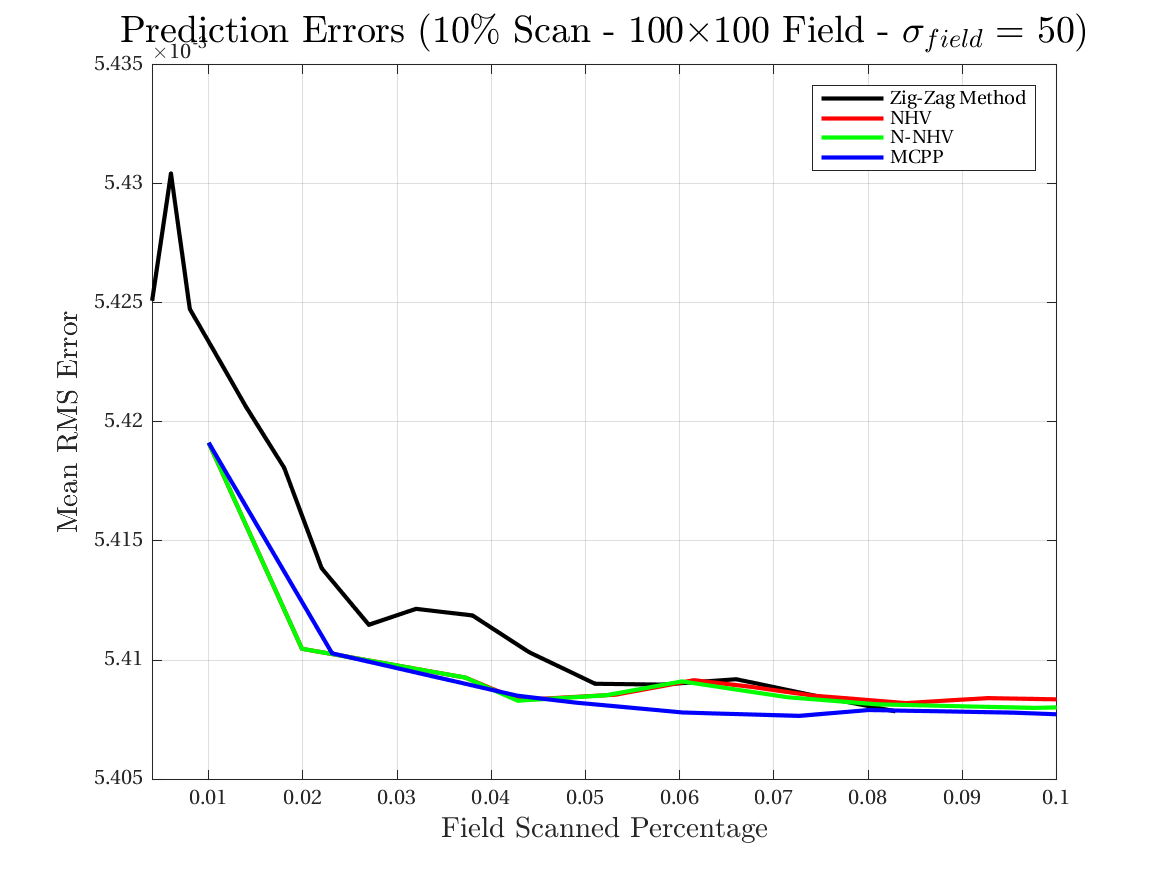
\includegraphics[width=\linewidth]{figures/hbresults/pred_errs_10p_100x100_sf_50_seed_3.png}
        \captionsetup{skip=0.20\baselineskip,size=footnotesize}
        \caption{Prediction errors (erf$(Z,\hat{Z})$).}
        \label{fig:prederrs_sigma50_p10_s3}
    \end{subfigure}%
    \\
    \begin{subfigure}[t]{0.65\textwidth}
        \centering
        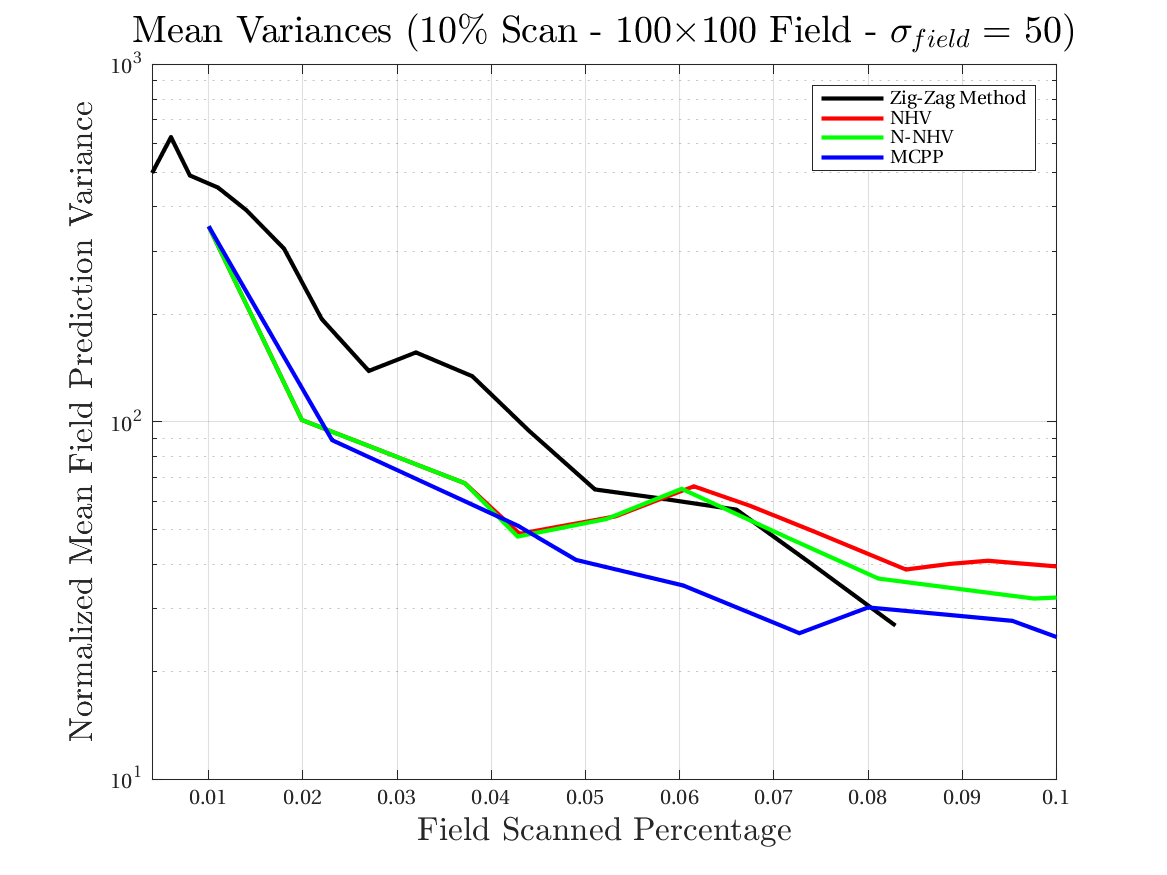
\includegraphics[width=\linewidth]{figures/hbresults/vars_10p_100x100_sf_50_seed_3.png}
        \captionsetup{skip=0.20\baselineskip,size=footnotesize}
        \caption{Semi-logarithmic prediction variances normalized to an a priori mean variance for the field.}
        \label{fig:prederrs_sigma50_p10_s3}
    \end{subfigure}
    \captionsetup{skip=0.20\baselineskip}
    \caption{A $10\%$ maximum area scan on a field of size $100 \times 100$, $\sigma_{field} = 50$, random seed: 3.}
    \label{fig:sigma50_p10_s3}
\end{figure}

\begin{figure}[htb!]
    \centering
    \begin{subfigure}[t]{0.5\textwidth}
        \centering
        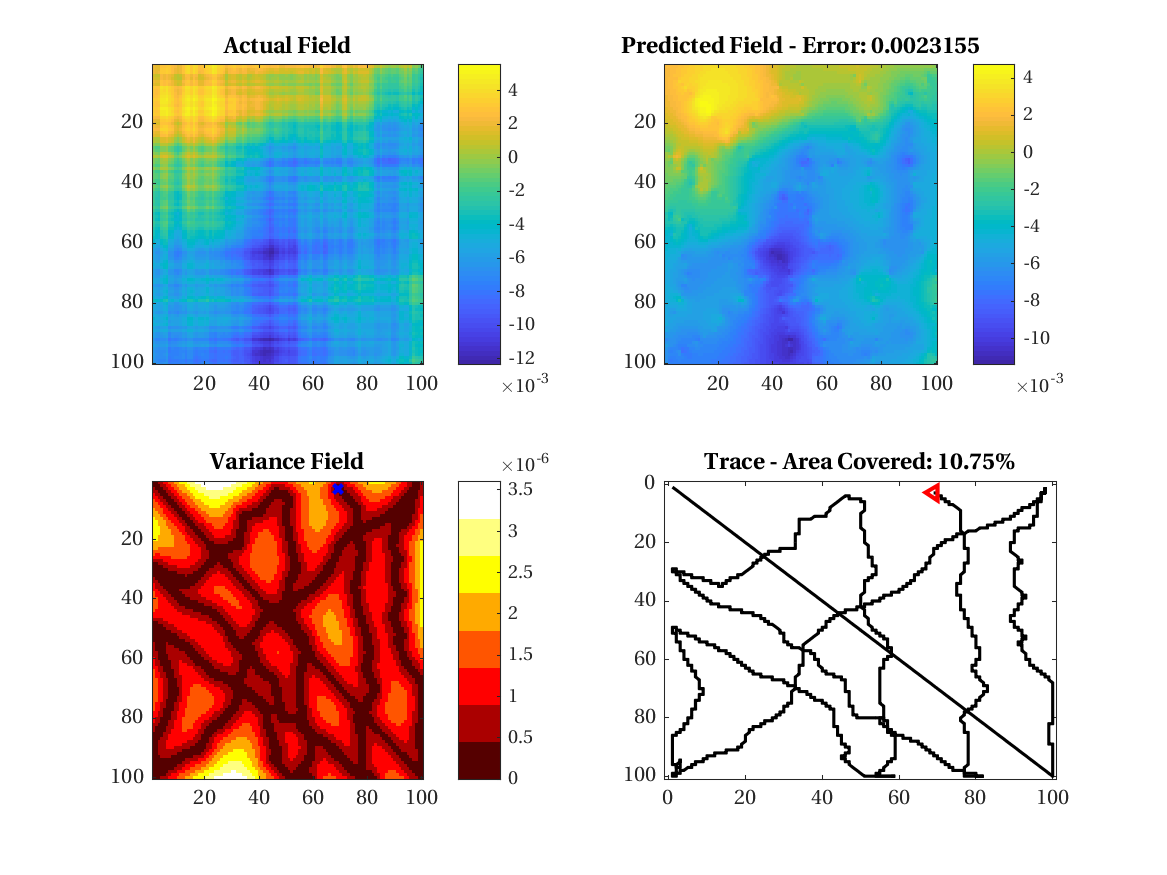
\includegraphics[width=\linewidth]{figures/hbresults/mc_10p_100x100_sf_50_seed_3.png}
        \captionsetup{skip=0.10\baselineskip,size=footnotesize}
        \caption{Monte Carlo Path Planner}
    \end{subfigure}%
    ~ 
    \begin{subfigure}[t]{0.5\textwidth}
        \centering
        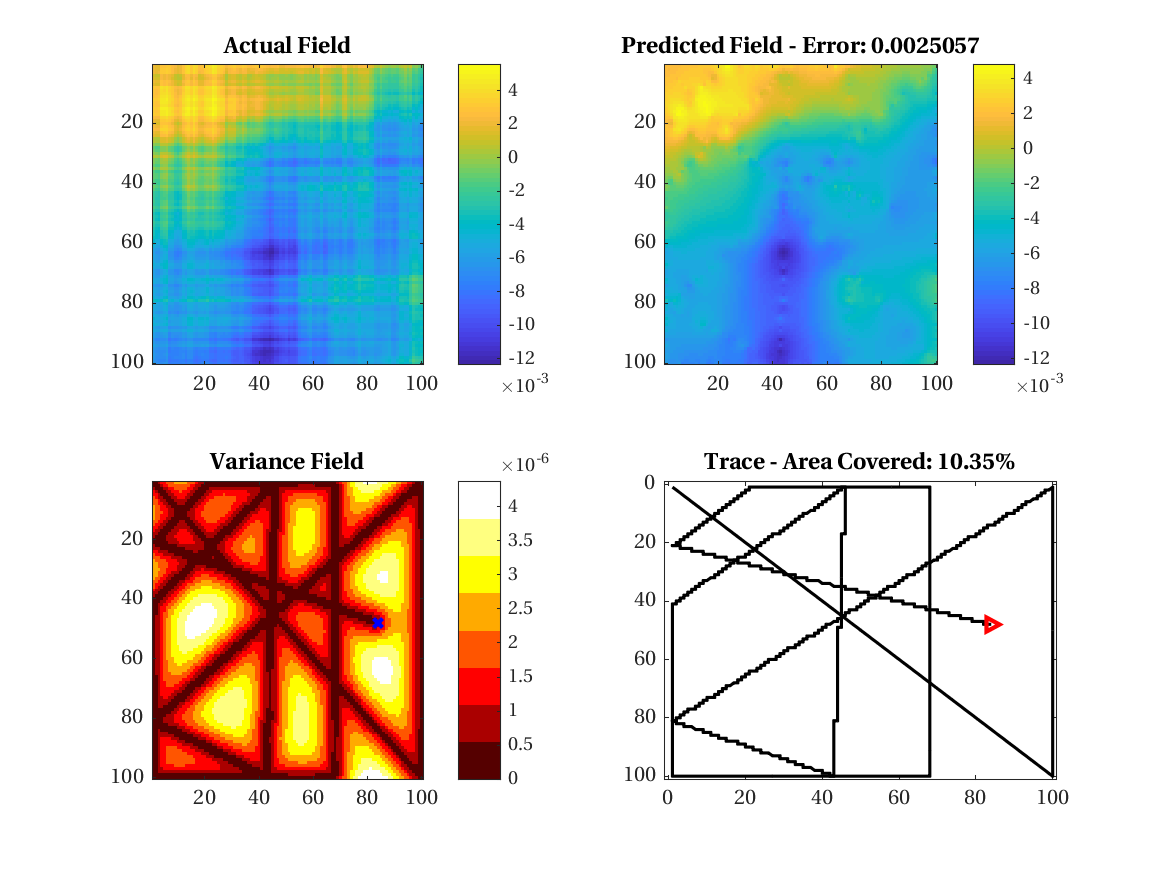
\includegraphics[width=\linewidth]{figures/hbresults/nhv_10p_100x100_sf_50_seed_3.png}
        \captionsetup{skip=0.10\baselineskip,size=footnotesize}
        \caption{Next Highest Variance Path Planner}
    \end{subfigure}%
    \\
    \begin{subfigure}[t]{0.5\textwidth}
        \centering
        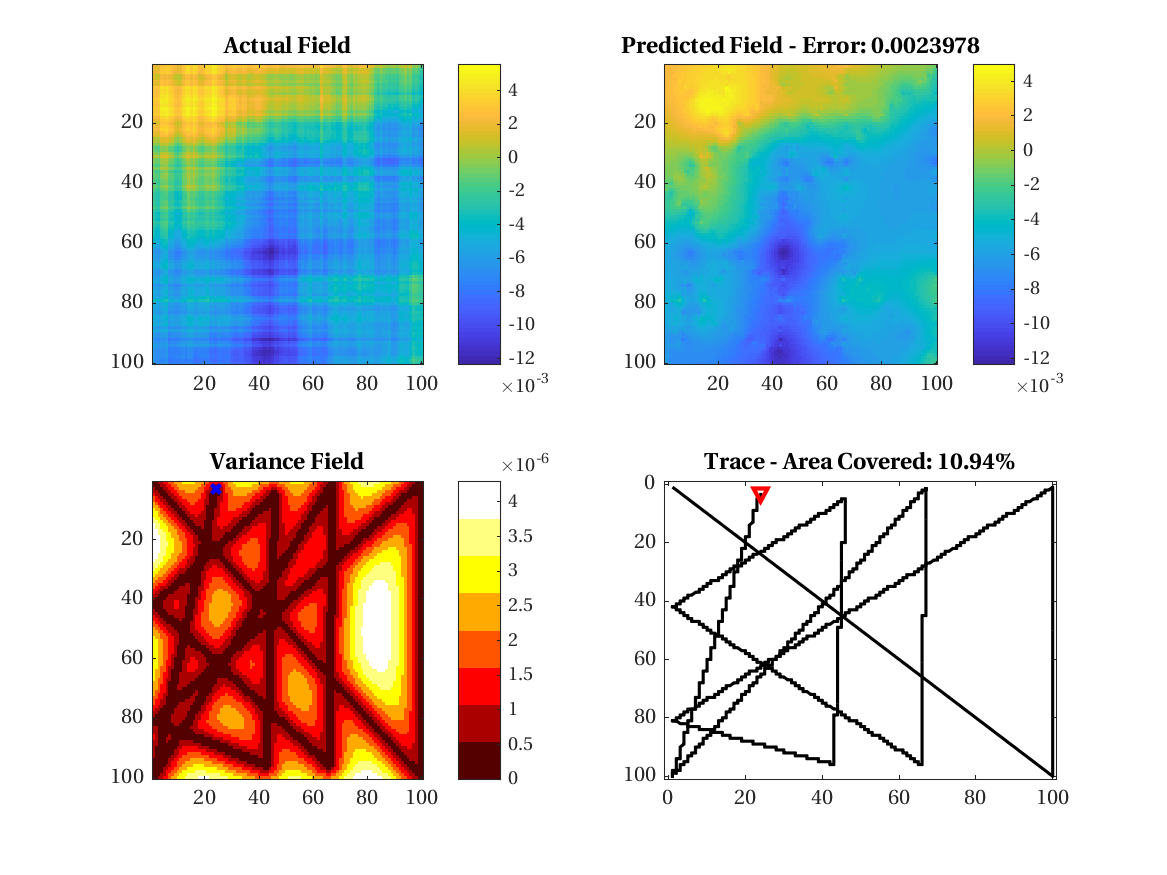
\includegraphics[width=\linewidth]{figures/hbresults/nnhv_10p_100x100_sf_50_seed_3.png}
        \captionsetup{skip=0.10\baselineskip,size=footnotesize}
        \caption{$N$ Next Highest Variance Path Planner}
    \end{subfigure}%
    ~
    \begin{subfigure}[t]{0.5\textwidth}
        \centering
        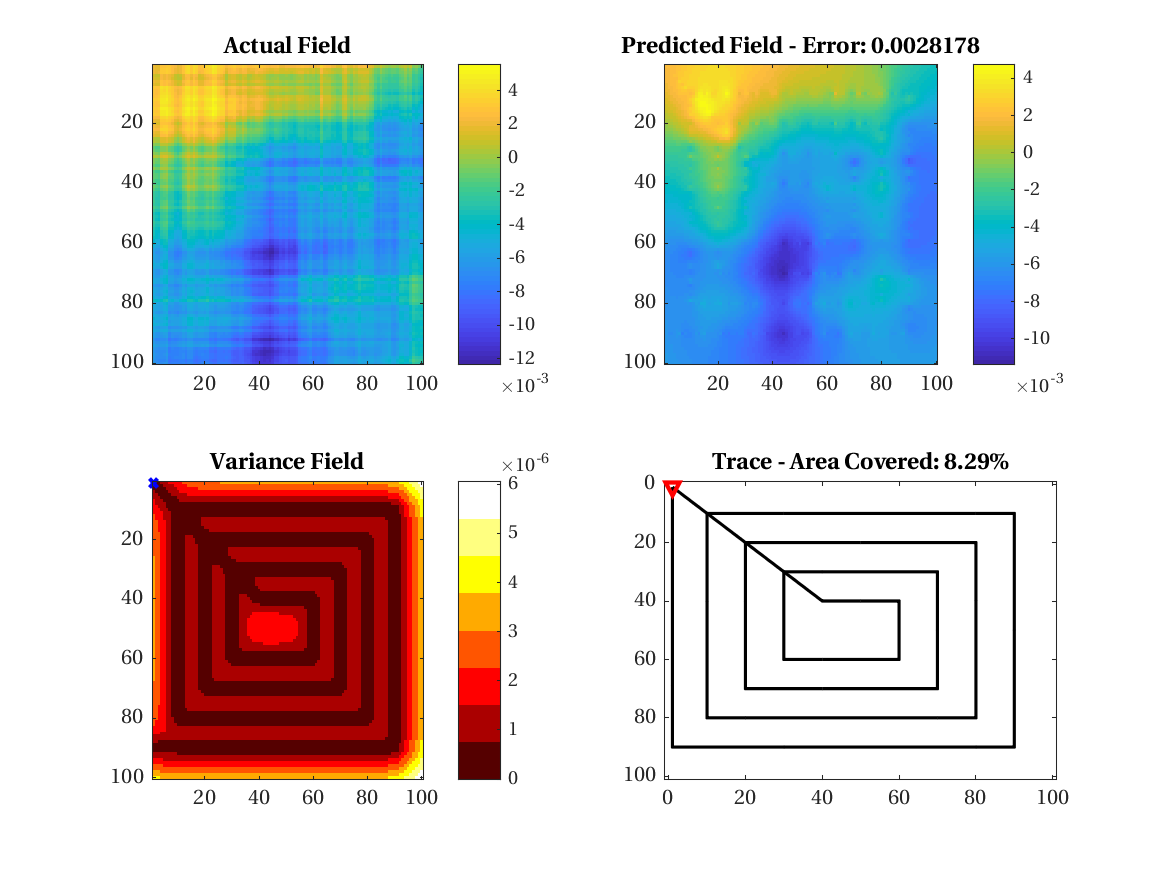
\includegraphics[width=\linewidth]{figures/hbresults/zz_10p_100x100_sf_50_seed_3.png}
        \captionsetup{skip=0.10\baselineskip,size=footnotesize}
        \caption{Zig-Zag Method}
    \end{subfigure}%
    \captionsetup{skip=0.20\baselineskip}
    \caption{Simulation output for a $10\%$ maximum area scan on a field of size $100 \times 100$, $\sigma_{field} = 50$, random seed: 3.}
    \label{fig:sim_sigma50_p10_s3}
\end{figure}

\FloatBarrier
\clearpage
\subsection{$20\%$ Maximum Field Scan}
\begin{figure}[htb!]
    \centering
    \begin{subfigure}[t]{0.65\textwidth}
        \centering
        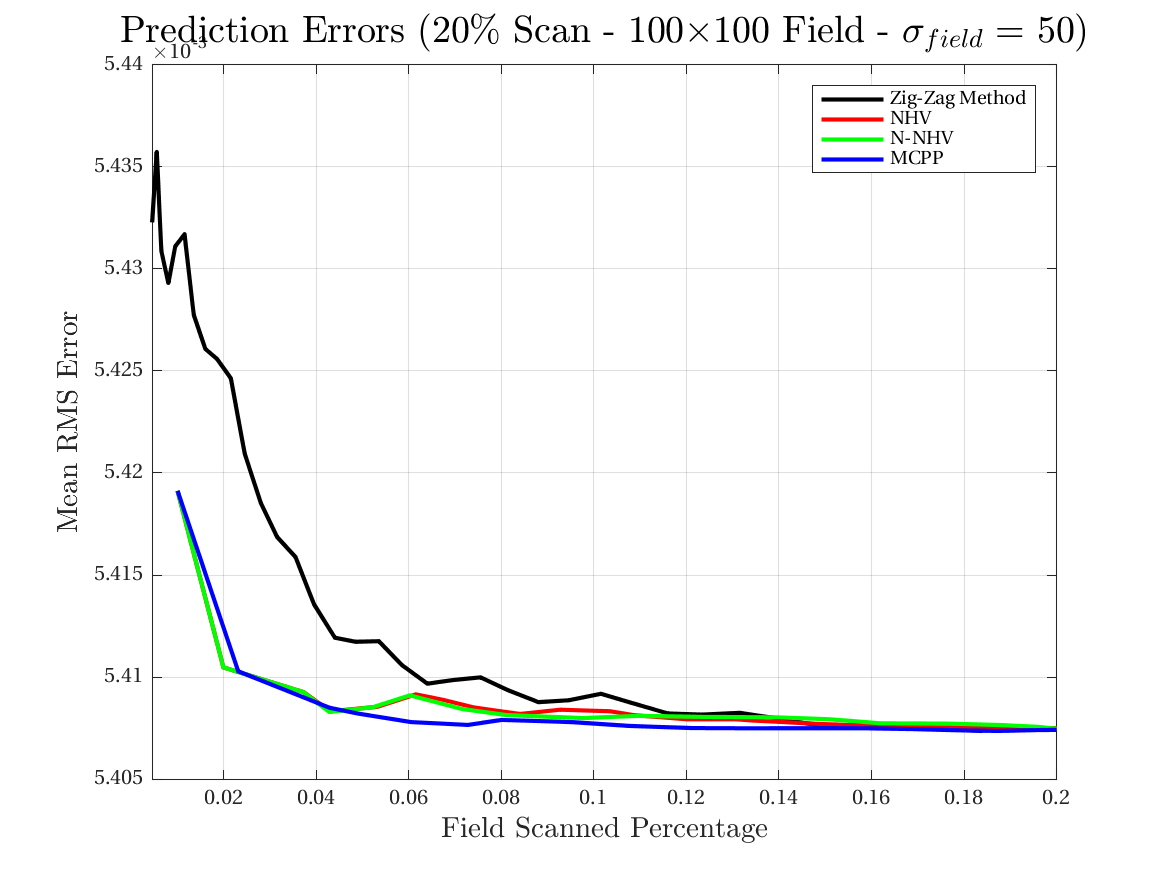
\includegraphics[width=\linewidth]{figures/hbresults/pred_errs_20p_100x100_sf_50_seed_3.png}
        \captionsetup{skip=0.20\baselineskip,size=footnotesize}
        \caption{Prediction errors (erf$(Z,\hat{Z})$).}
        \label{fig:prederrs_sigma50_p20_s3}
    \end{subfigure}%
    \\
    \begin{subfigure}[t]{0.65\textwidth}
        \centering
        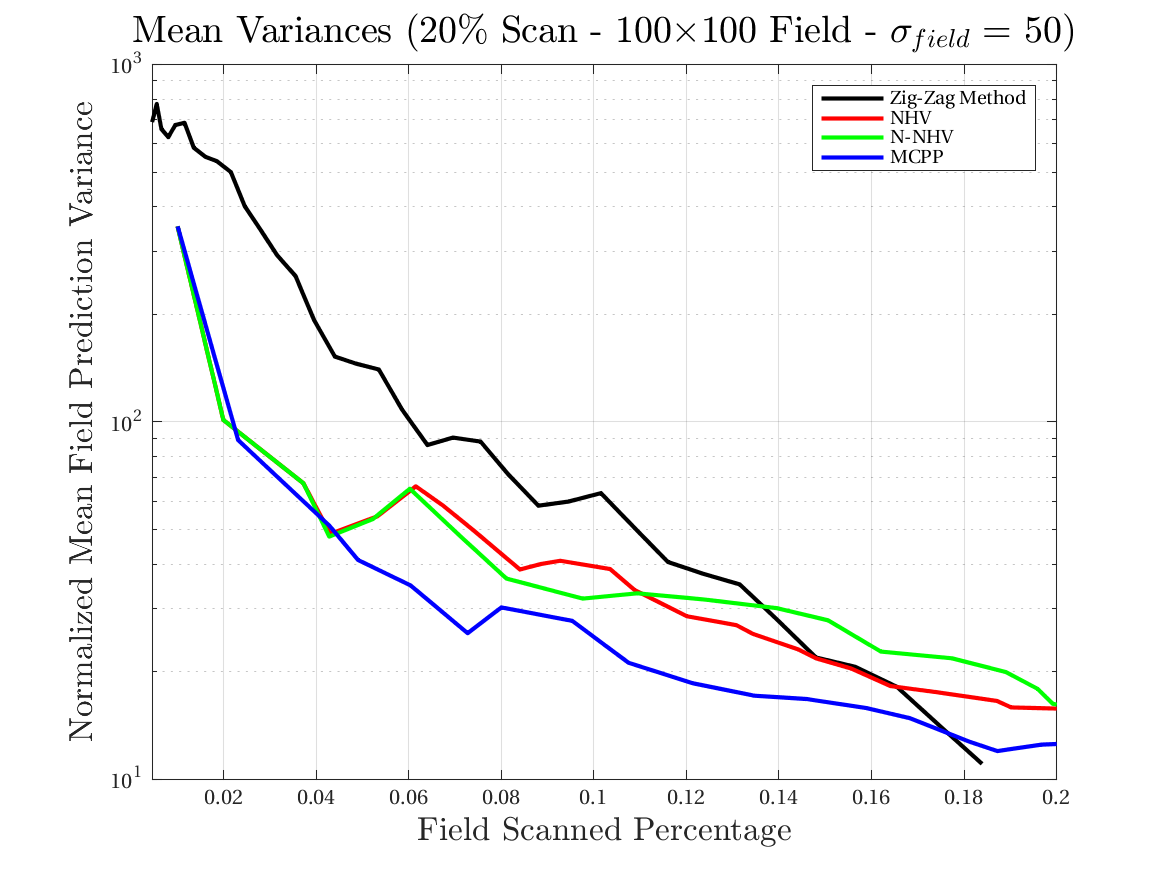
\includegraphics[width=\linewidth]{figures/hbresults/vars_20p_100x100_sf_50_seed_3.png}
        \captionsetup{skip=0.20\baselineskip,size=footnotesize}
        \caption{Semi-logarithmic prediction variances normalized to an a priori mean variance for the field.}
        \label{fig:prederrs_sigma50_p20_s3}
    \end{subfigure}
    \captionsetup{skip=0.20\baselineskip}
    \caption{A $20\%$ maximum area scan on a field of size $100 \times 100$, $\sigma_{field} = 50$, random seed: 3.}
    \label{fig:sigma50_p20_s3}
\end{figure}

\begin{figure}[htb!]
    \centering
    \begin{subfigure}[t]{0.5\textwidth}
        \centering
        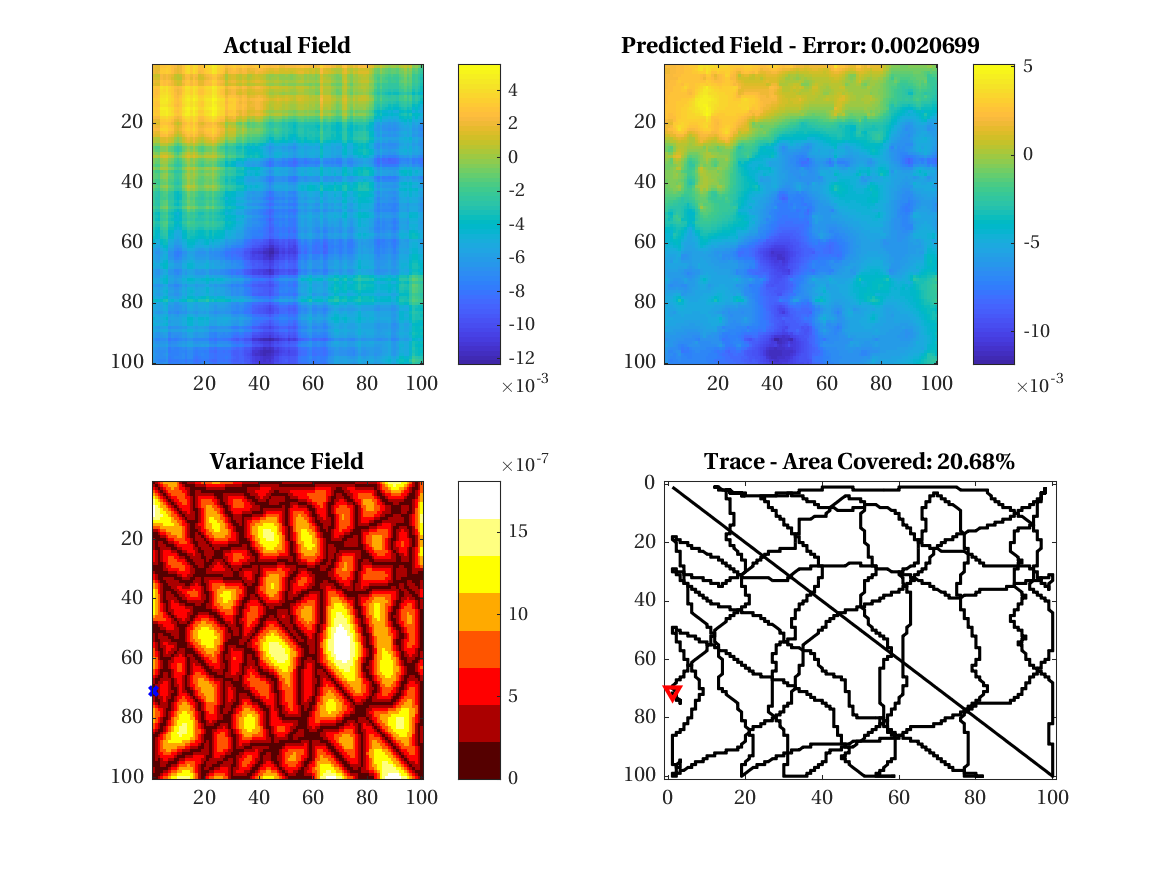
\includegraphics[width=\linewidth]{figures/hbresults/mc_20p_100x100_sf_50_seed_3.png}
        \captionsetup{skip=0.10\baselineskip,size=footnotesize}
        \caption{Monte Carlo Path Planner}
    \end{subfigure}%
    ~ 
    \begin{subfigure}[t]{0.5\textwidth}
        \centering
        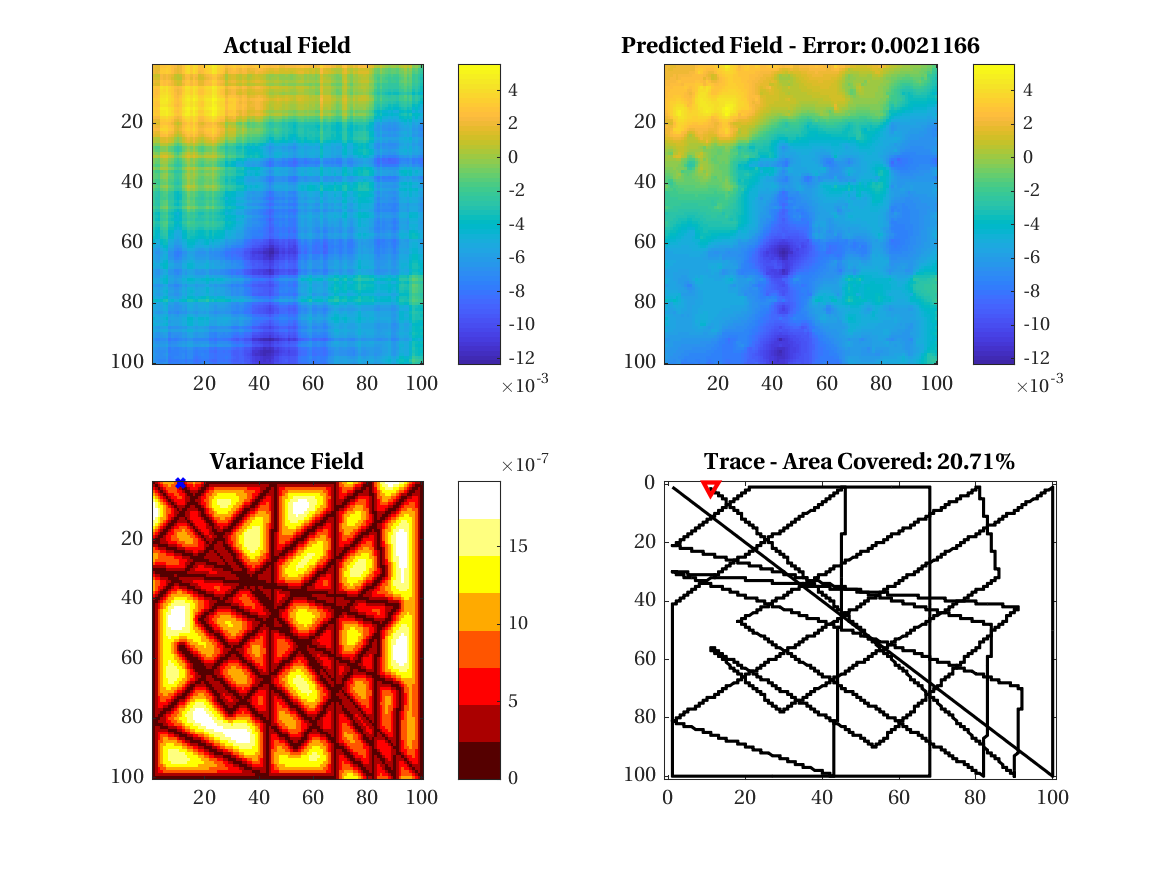
\includegraphics[width=\linewidth]{figures/hbresults/nhv_20p_100x100_sf_50_seed_3.png}
        \captionsetup{skip=0.10\baselineskip,size=footnotesize}
        \caption{Next Highest Variance Path Planner}
    \end{subfigure}%
    \\
    \begin{subfigure}[t]{0.5\textwidth}
        \centering
        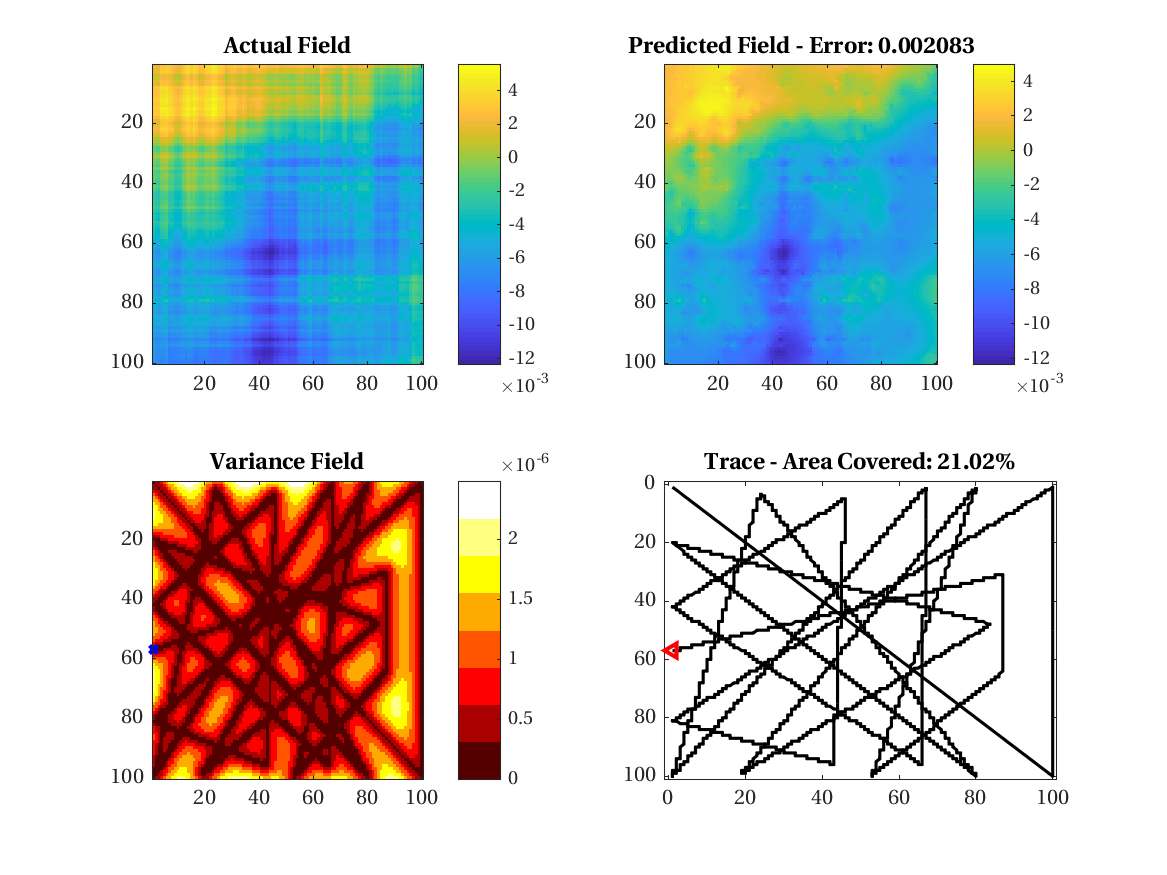
\includegraphics[width=\linewidth]{figures/hbresults/nnhv_20p_100x100_sf_50_seed_3.png}
        \captionsetup{skip=0.10\baselineskip,size=footnotesize}
        \caption{$N$ Next Highest Variance Path Planner}
    \end{subfigure}%
    ~
    \begin{subfigure}[t]{0.5\textwidth}
        \centering
        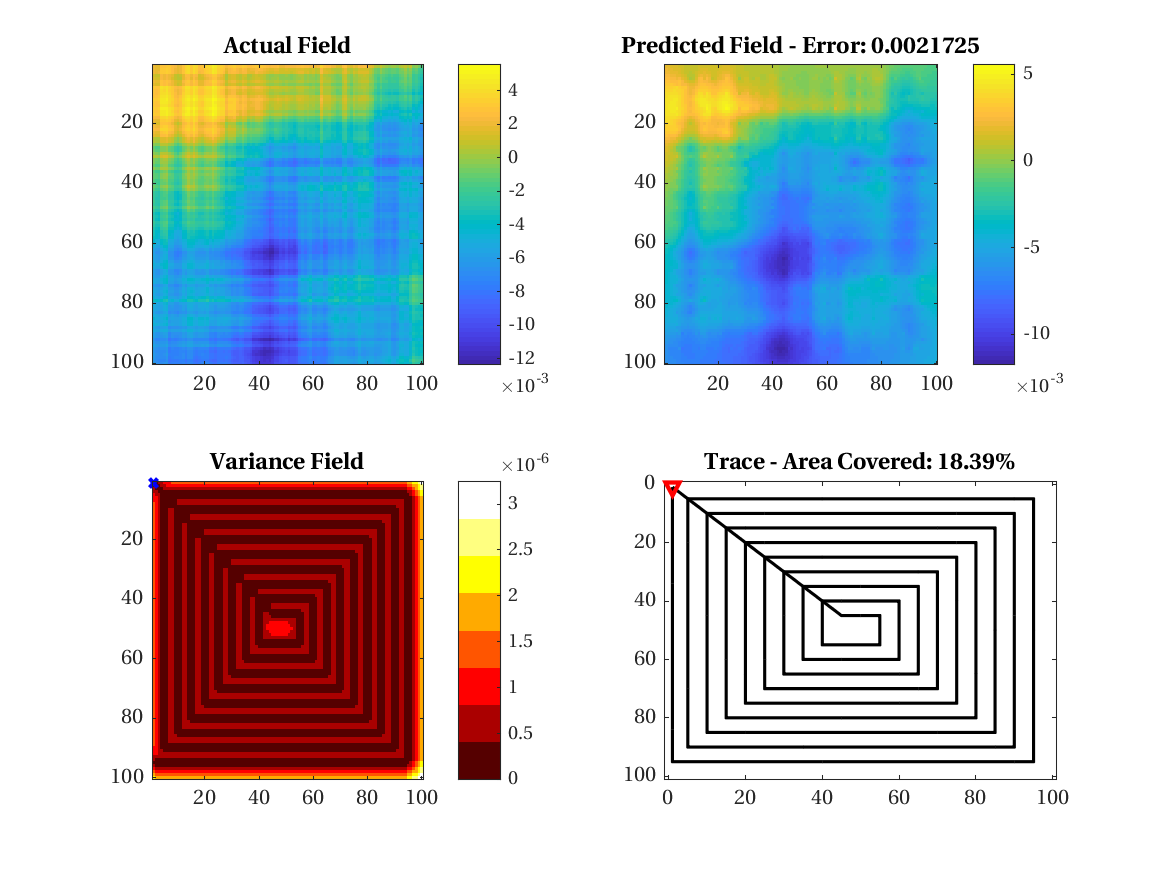
\includegraphics[width=\linewidth]{figures/hbresults/zz_20p_100x100_sf_50_seed_3.png}
        \captionsetup{skip=0.10\baselineskip,size=footnotesize}
        \caption{Zig-Zag Method}
    \end{subfigure}%
    \captionsetup{skip=0.20\baselineskip}
    \caption{Simulation output for a $20\%$ maximum area scan on a field of size $100 \times 100$, $\sigma_{field} = 50$, random seed: 3.}
    \label{fig:sim_sigma50_p20_s3}
\end{figure}

\FloatBarrier
\clearpage
\subsection{$30\%$ Maximum Field Scan}
\begin{figure}[htb!]
    \centering
    \begin{subfigure}[t]{0.65\textwidth}
        \centering
        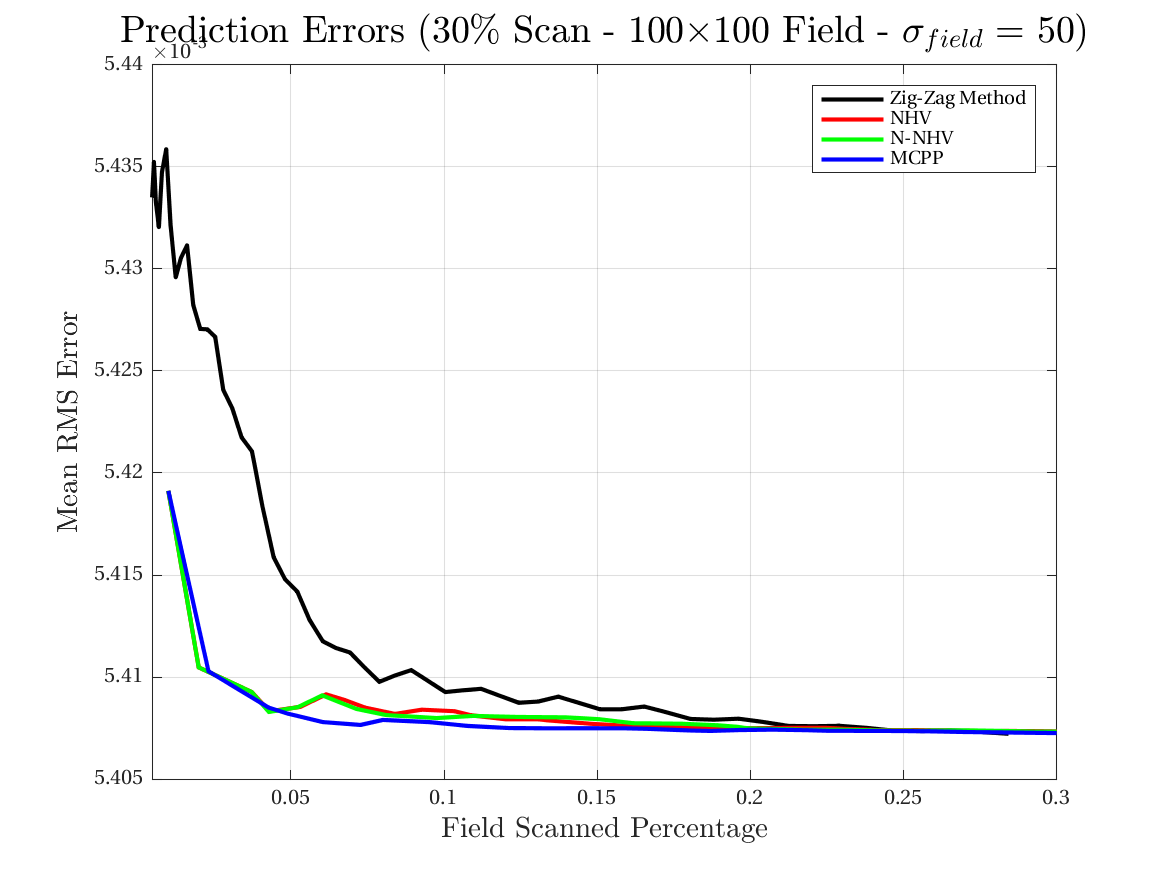
\includegraphics[width=\linewidth]{figures/hbresults/pred_errs_30p_100x100_sf_50_seed_3.png}
        \captionsetup{skip=0.20\baselineskip,size=footnotesize}
        \caption{Prediction errors (erf$(Z,\hat{Z})$).}
        \label{fig:prederrs_sigma50_p30_s3}
    \end{subfigure}%
    \\
    \begin{subfigure}[t]{0.65\textwidth}
        \centering
        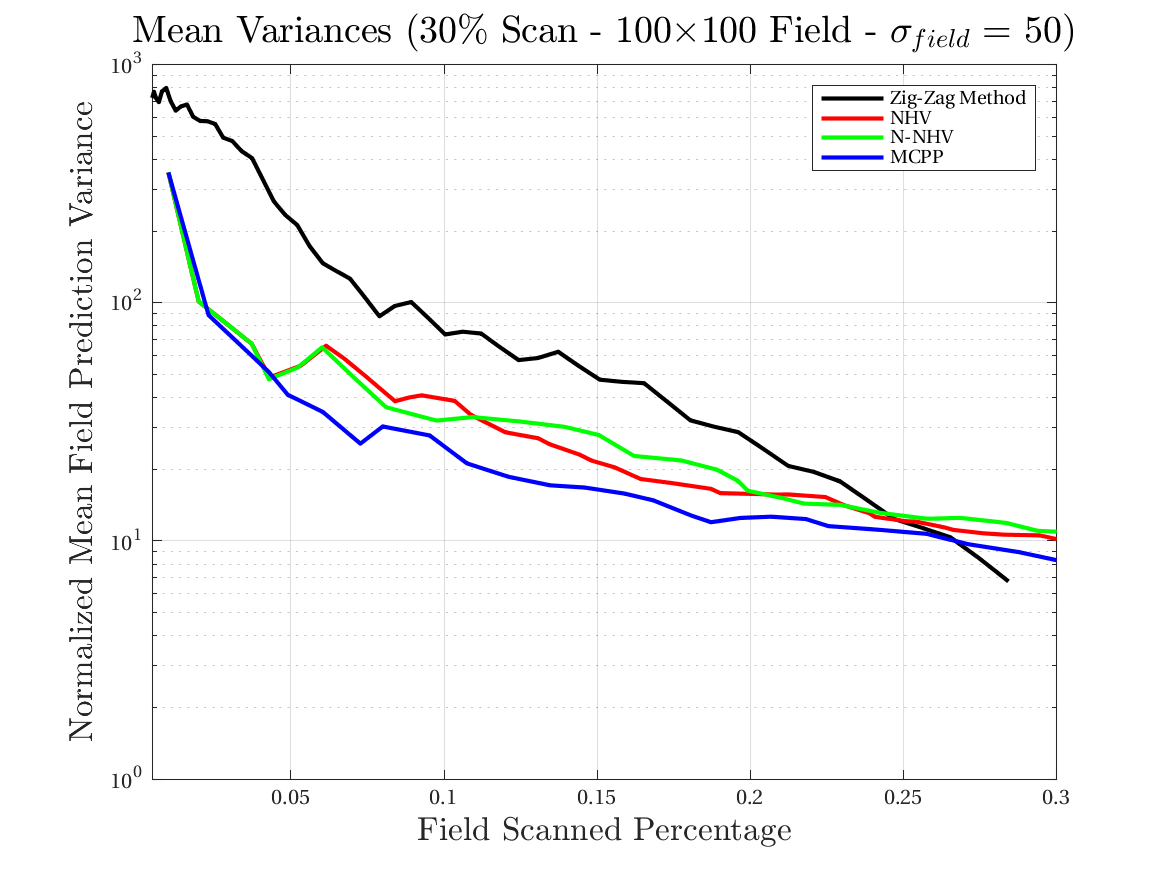
\includegraphics[width=\linewidth]{figures/hbresults/vars_30p_100x100_sf_50_seed_3.png}
        \captionsetup{skip=0.20\baselineskip,size=footnotesize}
        \caption{Semi-logarithmic prediction variances normalized to an a priori mean variance for the field.}
        \label{fig:prederrs_sigma50_p30_s3}
    \end{subfigure}
    \captionsetup{skip=0.20\baselineskip}
    \caption{A $30\%$ maximum area scan on a field of size $100 \times 100$, $\sigma_{field} = 50$, random seed: 3.}
    \label{fig:sigma50_p30_s3}
\end{figure}

\begin{figure}[htb!]
    \centering
    \begin{subfigure}[t]{0.5\textwidth}
        \centering
        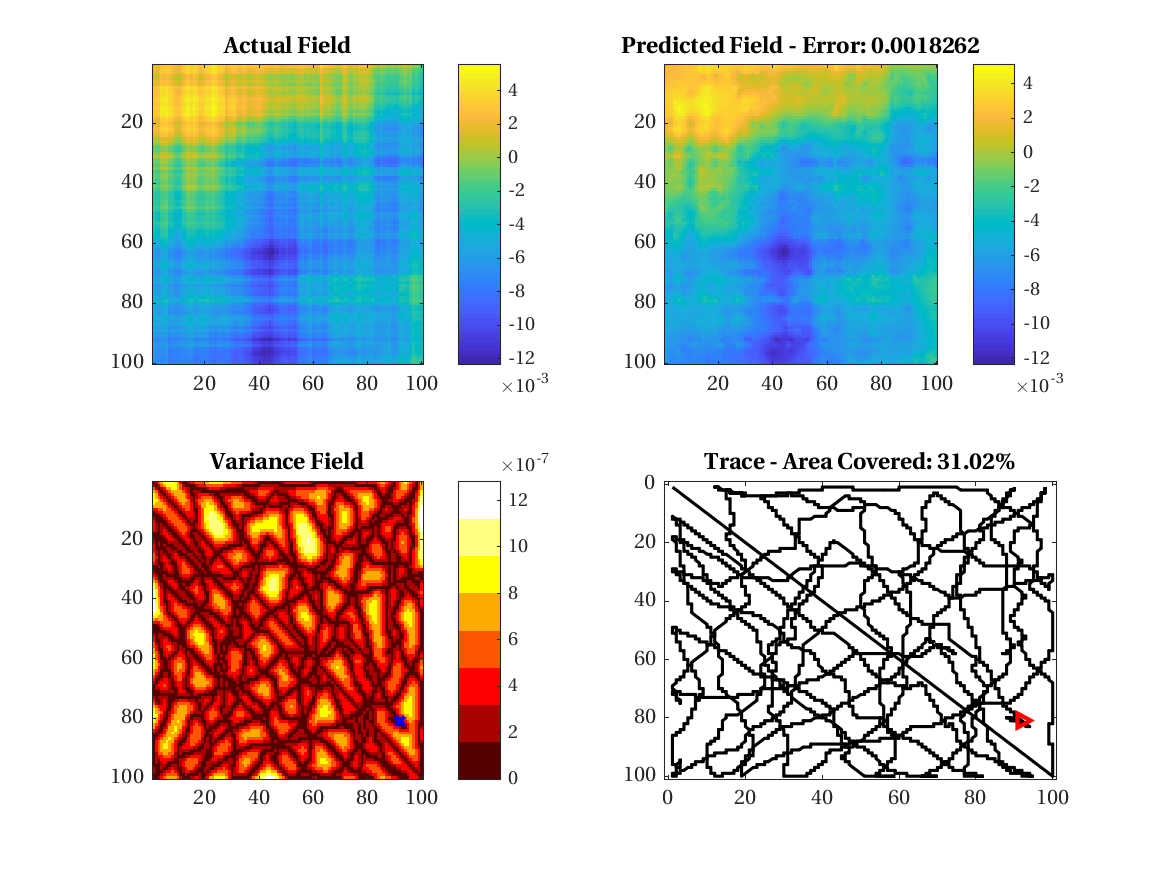
\includegraphics[width=\linewidth]{figures/hbresults/mc_30p_100x100_sf_50_seed_3.png}
        \captionsetup{skip=0.10\baselineskip,size=footnotesize}
        \caption{Monte Carlo Path Planner}
    \end{subfigure}%
    ~ 
    \begin{subfigure}[t]{0.5\textwidth}
        \centering
        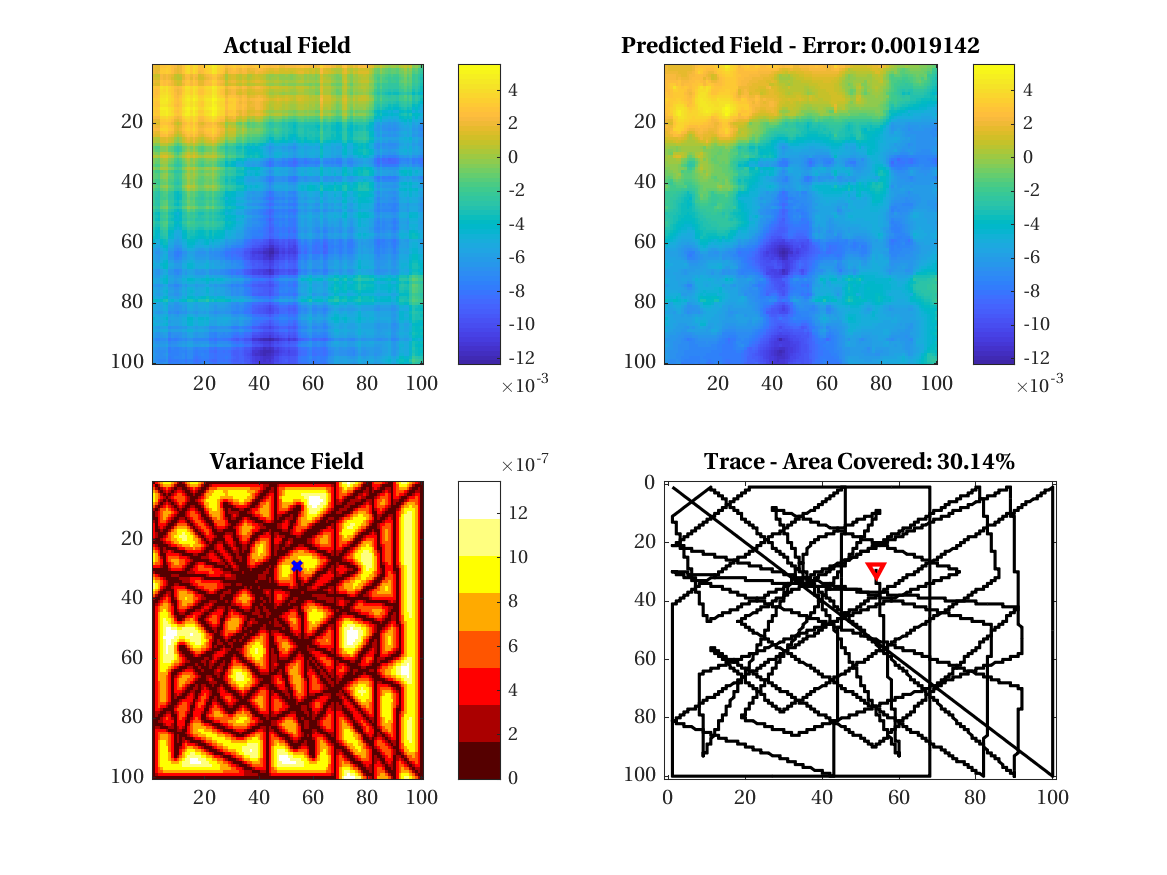
\includegraphics[width=\linewidth]{figures/hbresults/nhv_30p_100x100_sf_50_seed_3.png}
        \captionsetup{skip=0.10\baselineskip,size=footnotesize}
        \caption{Next Highest Variance Path Planner}
    \end{subfigure}%
    \\
    \begin{subfigure}[t]{0.5\textwidth}
        \centering
        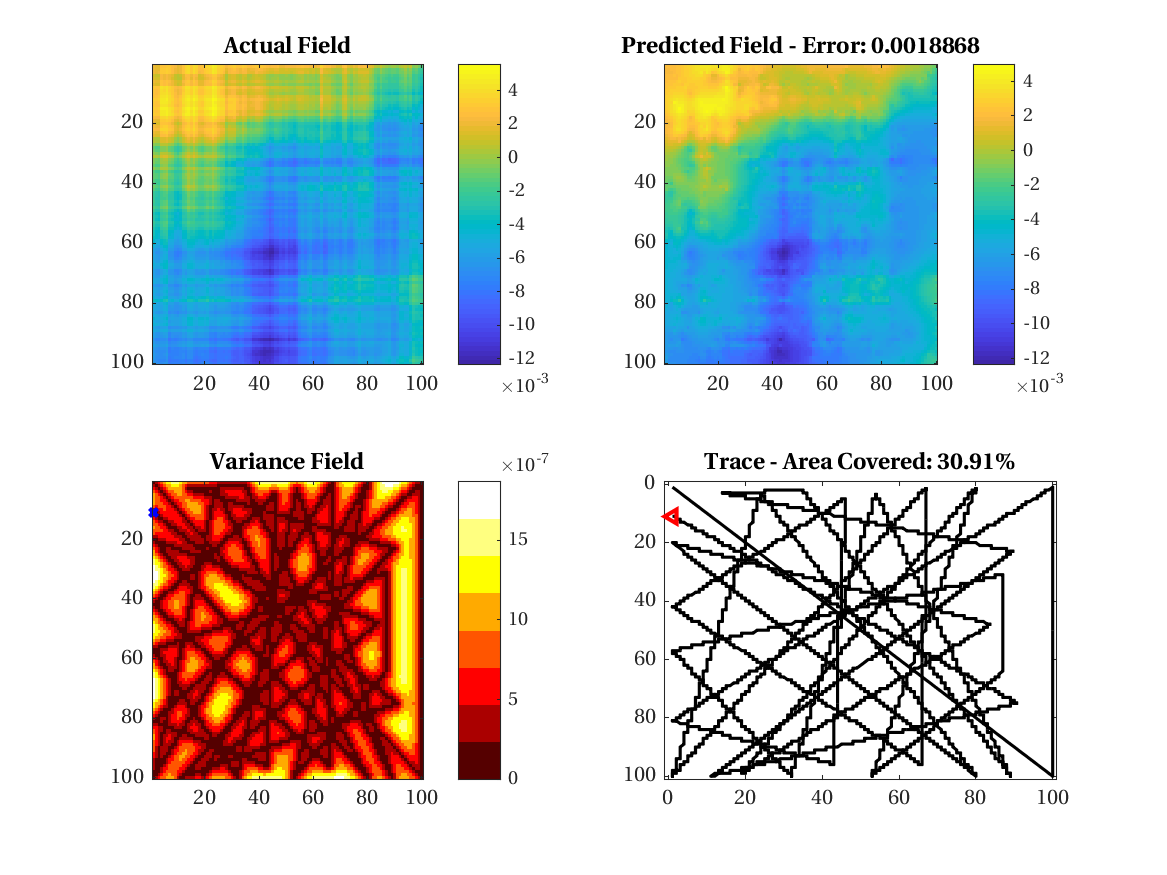
\includegraphics[width=\linewidth]{figures/hbresults/nnhv_30p_100x100_sf_50_seed_3.png}
        \captionsetup{skip=0.10\baselineskip,size=footnotesize}
        \caption{$N$ Next Highest Variance Path Planner}
    \end{subfigure}%
    ~
    \begin{subfigure}[t]{0.5\textwidth}
        \centering
        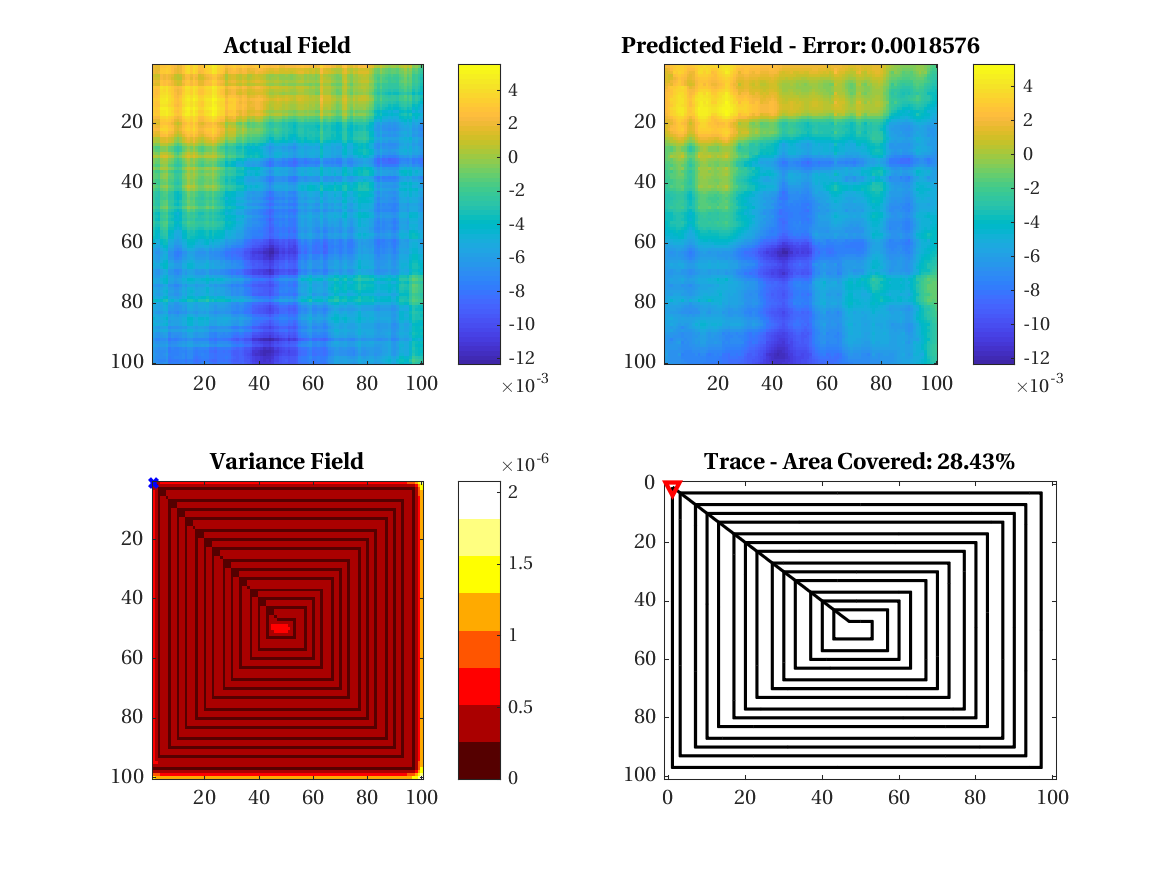
\includegraphics[width=\linewidth]{figures/hbresults/zz_30p_100x100_sf_50_seed_3.png}
        \captionsetup{skip=0.10\baselineskip,size=footnotesize}
        \caption{Zig-Zag Method}
    \end{subfigure}%
    \captionsetup{skip=0.20\baselineskip}
    \caption{Simulation output for a $30\%$ maximum area scan on a field of size $100 \times 100$, $\sigma_{field} = 50$, random seed: 3.}
    \label{fig:sim_sigma50_p30_s3}
\end{figure}
%% SIGMA QUARTER

\section{Quarter Width Spatial Autocorrelation Results}
The methods will be compared on target fields generated with an autocorrelation factor, $\sigma_{field}$, that is one quarter of the field width.

\clearpage
\subsection{$10\%$ Maximum Field Scan}
\begin{figure}[htb!]
    \centering
    \begin{subfigure}[t]{0.65\textwidth}
        \centering
        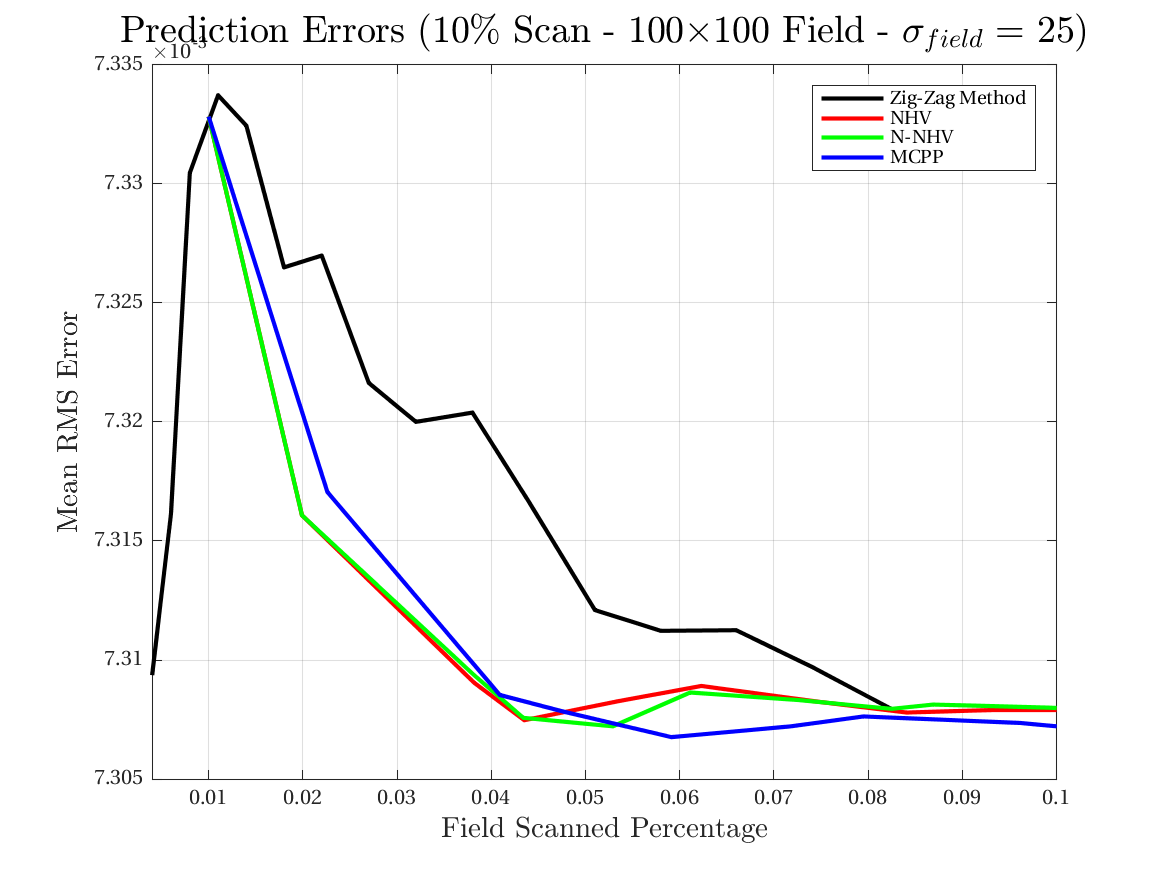
\includegraphics[width=\linewidth]{figures/hbresults/pred_errs_10p_100x100_sf_25_seed_3.png}
        \captionsetup{skip=0.20\baselineskip,size=footnotesize}
        \caption{Prediction errors (erf$(Z,\hat{Z})$).}
        \label{fig:prederrs_sigma25_p10_s3}
    \end{subfigure}%
    \\
    \begin{subfigure}[t]{0.65\textwidth}
        \centering
        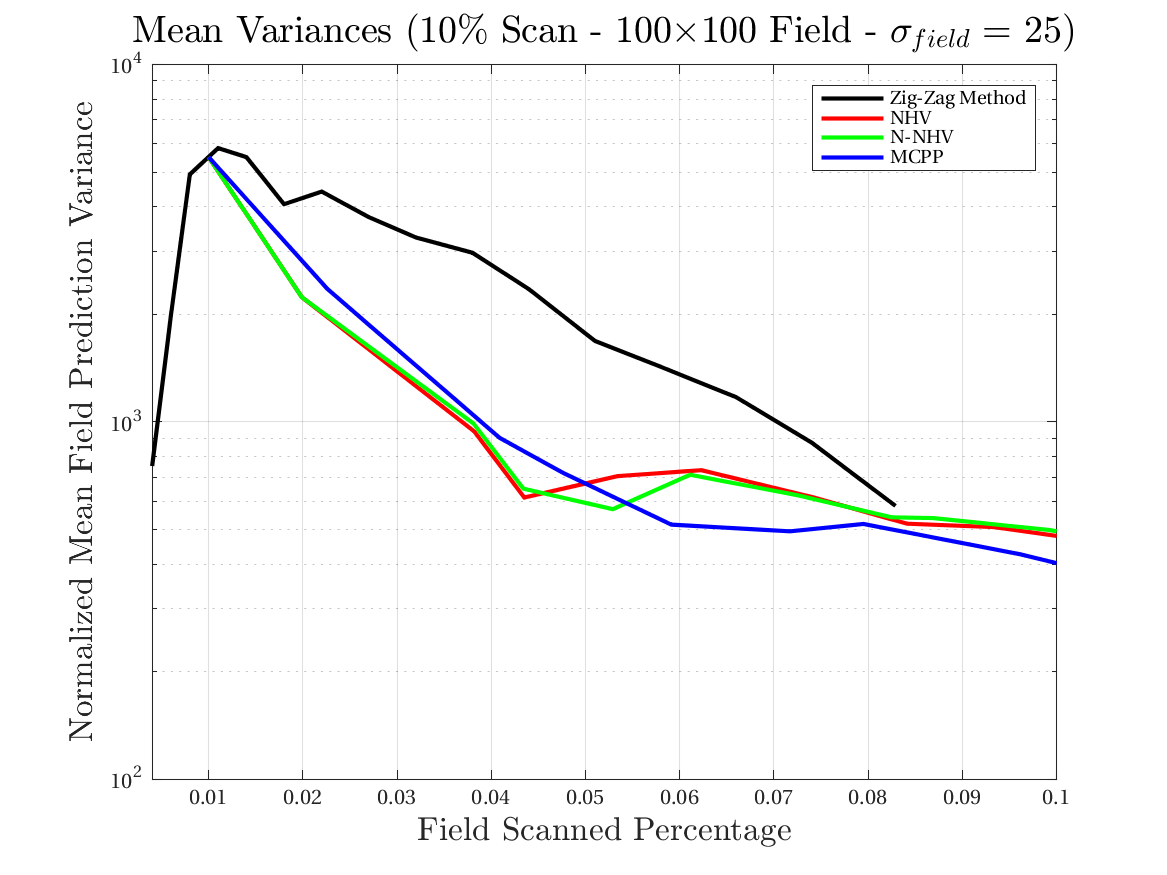
\includegraphics[width=\linewidth]{figures/hbresults/vars_10p_100x100_sf_25_seed_3.png}
        \captionsetup{skip=0.20\baselineskip,size=footnotesize}
        \caption{Semi-logarithmic prediction variances normalized to an a priori mean variance for the field.}
        \label{fig:prederrs_sigma25_p10_s3}
    \end{subfigure}
    \captionsetup{skip=0.20\baselineskip}
    \caption{A $10\%$ maximum area scan on a field of size $100 \times 100$, $\sigma_{field} = 25$, random seed: 3.}
    \label{fig:sigma25_p10_s3}
\end{figure}

\begin{figure}[htb!]
    \centering
    \begin{subfigure}[t]{0.5\textwidth}
        \centering
        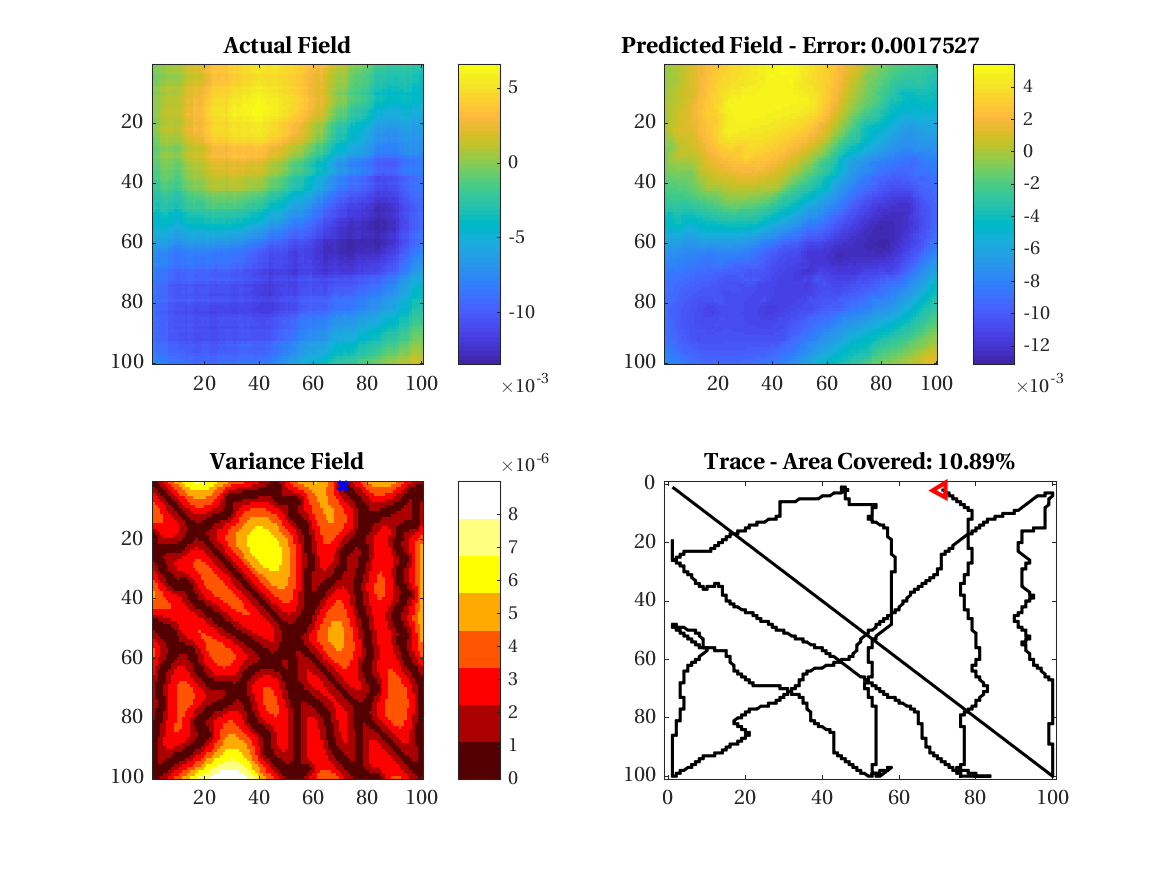
\includegraphics[width=\linewidth]{figures/hbresults/mc_10p_100x100_sf_25_seed_3.png}
        \captionsetup{skip=0.10\baselineskip,size=footnotesize}
        \caption{Monte Carlo Path Planner}
    \end{subfigure}%
    ~ 
    \begin{subfigure}[t]{0.5\textwidth}
        \centering
        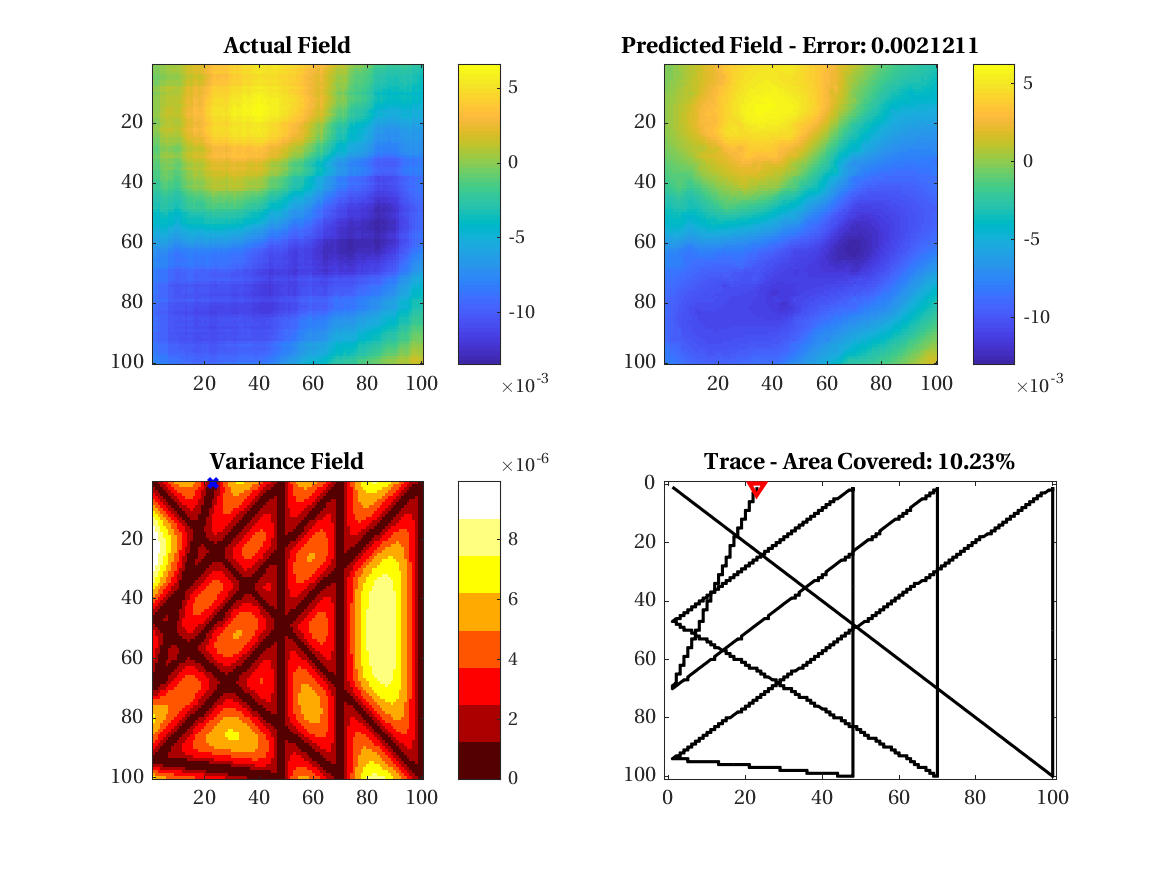
\includegraphics[width=\linewidth]{figures/hbresults/nhv_10p_100x100_sf_25_seed_3.png}
        \captionsetup{skip=0.10\baselineskip,size=footnotesize}
        \caption{Next Highest Variance Path Planner}
    \end{subfigure}%
    \\
    \begin{subfigure}[t]{0.5\textwidth}
        \centering
        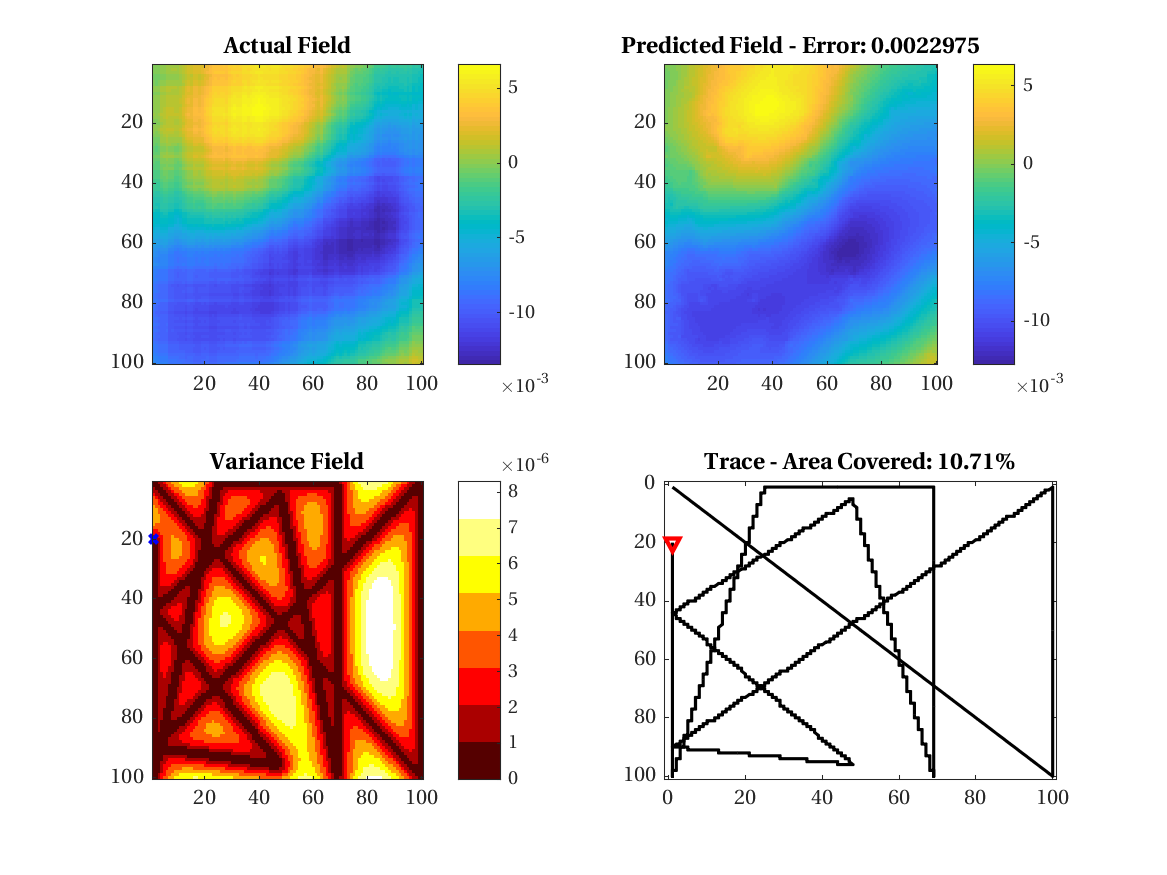
\includegraphics[width=\linewidth]{figures/hbresults/nnhv_10p_100x100_sf_25_seed_3.png}
        \captionsetup{skip=0.10\baselineskip,size=footnotesize}
        \caption{$N$ Next Highest Variance Path Planner}
    \end{subfigure}%
    ~
    \begin{subfigure}[t]{0.5\textwidth}
        \centering
        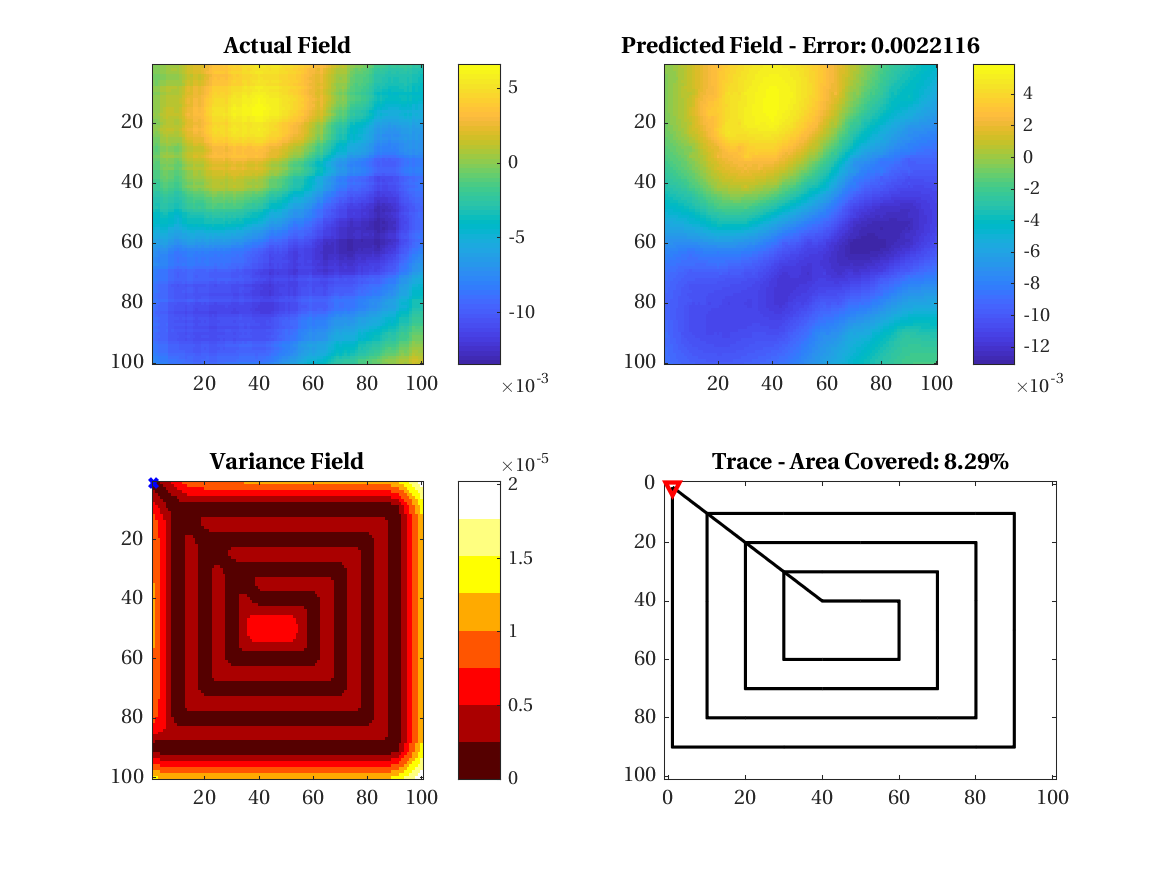
\includegraphics[width=\linewidth]{figures/hbresults/zz_10p_100x100_sf_25_seed_3.png}
        \captionsetup{skip=0.10\baselineskip,size=footnotesize}
        \caption{Zig-Zag Method}
    \end{subfigure}%
    \captionsetup{skip=0.20\baselineskip}
    \caption{Simulation output for a $10\%$ maximum area scan on a field of size $100 \times 100$, $\sigma_{field} = 25$, random seed: 3.}
    \label{fig:sim_sigma25_p10_s3}
\end{figure}

\FloatBarrier
\clearpage
\subsection{$20\%$ Maximum Field Scan}
\begin{figure}[htb!]
    \centering
    \begin{subfigure}[t]{0.65\textwidth}
        \centering
        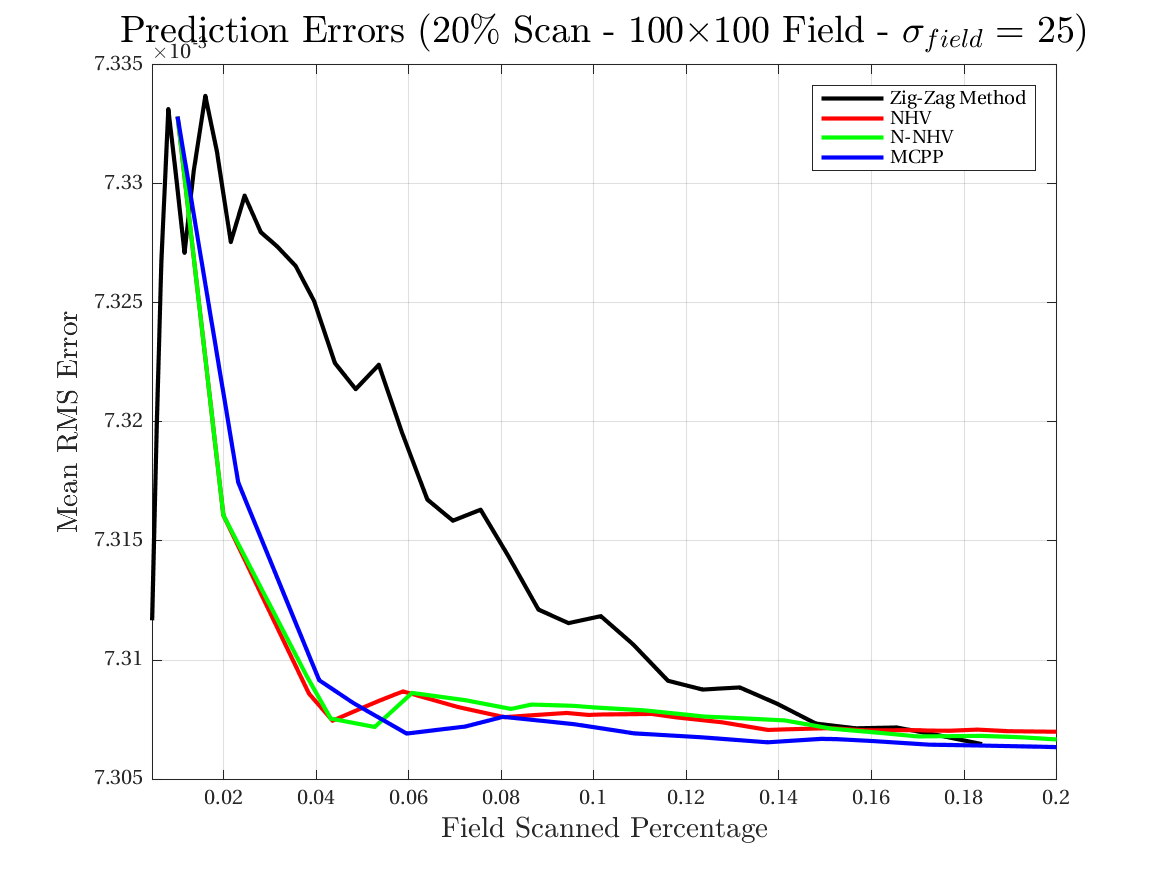
\includegraphics[width=\linewidth]{figures/hbresults/pred_errs_20p_100x100_sf_25_seed_3.png}
        \captionsetup{skip=0.20\baselineskip,size=footnotesize}
        \caption{Prediction errors (erf$(Z,\hat{Z})$).}
        \label{fig:prederrs_sigma25_p20_s3}
    \end{subfigure}%
    \\
    \begin{subfigure}[t]{0.65\textwidth}
        \centering
        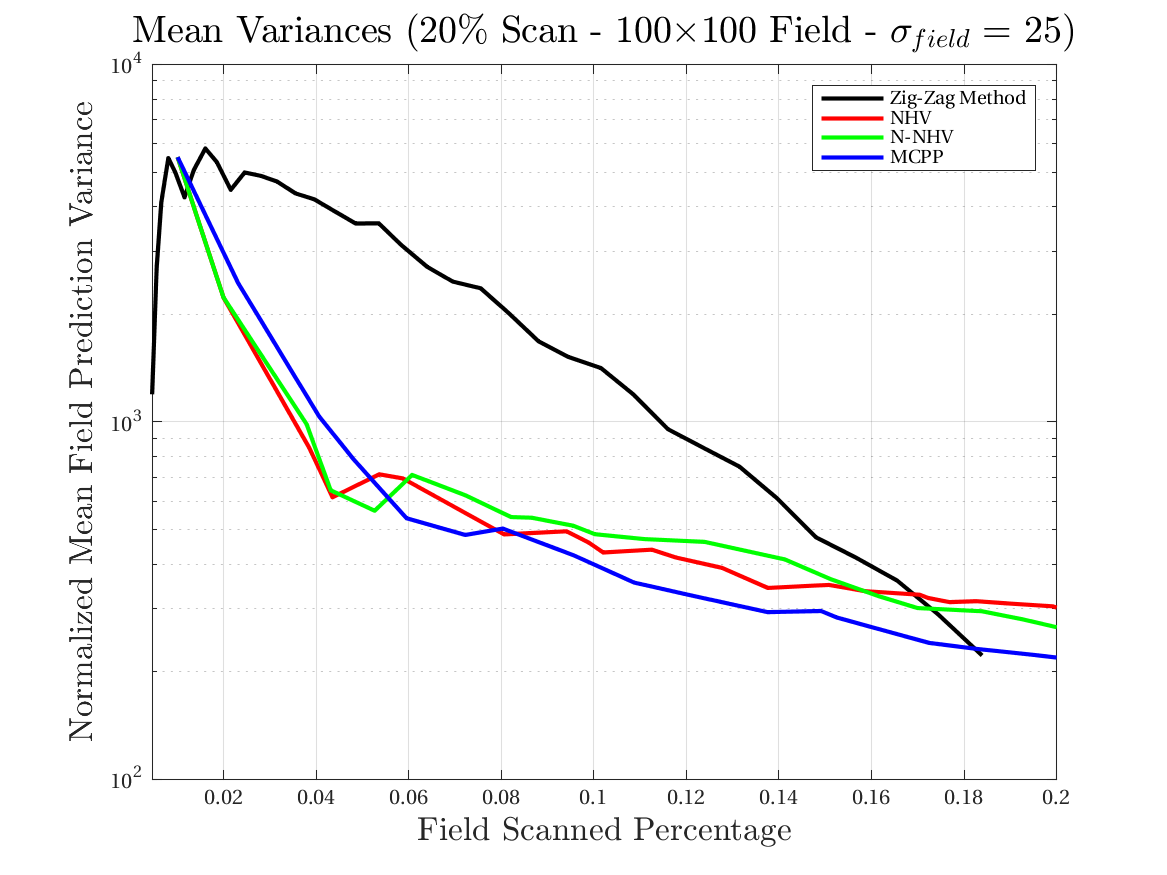
\includegraphics[width=\linewidth]{figures/hbresults/vars_20p_100x100_sf_25_seed_3.png}
        \captionsetup{skip=0.20\baselineskip,size=footnotesize}
        \caption{Semi-logarithmic prediction variances normalized to an a priori mean variance for the field.}
        \label{fig:prederrs_sigma25_p20_s3}
    \end{subfigure}
    \captionsetup{skip=0.20\baselineskip}
    \caption{A $20\%$ maximum area scan on a field of size $100 \times 100$, $\sigma_{field} = 25$, random seed: 3.}
    \label{fig:sigma25_p20_s3}
\end{figure}

\begin{figure}[htb!]
    \centering
    \begin{subfigure}[t]{0.5\textwidth}
        \centering
        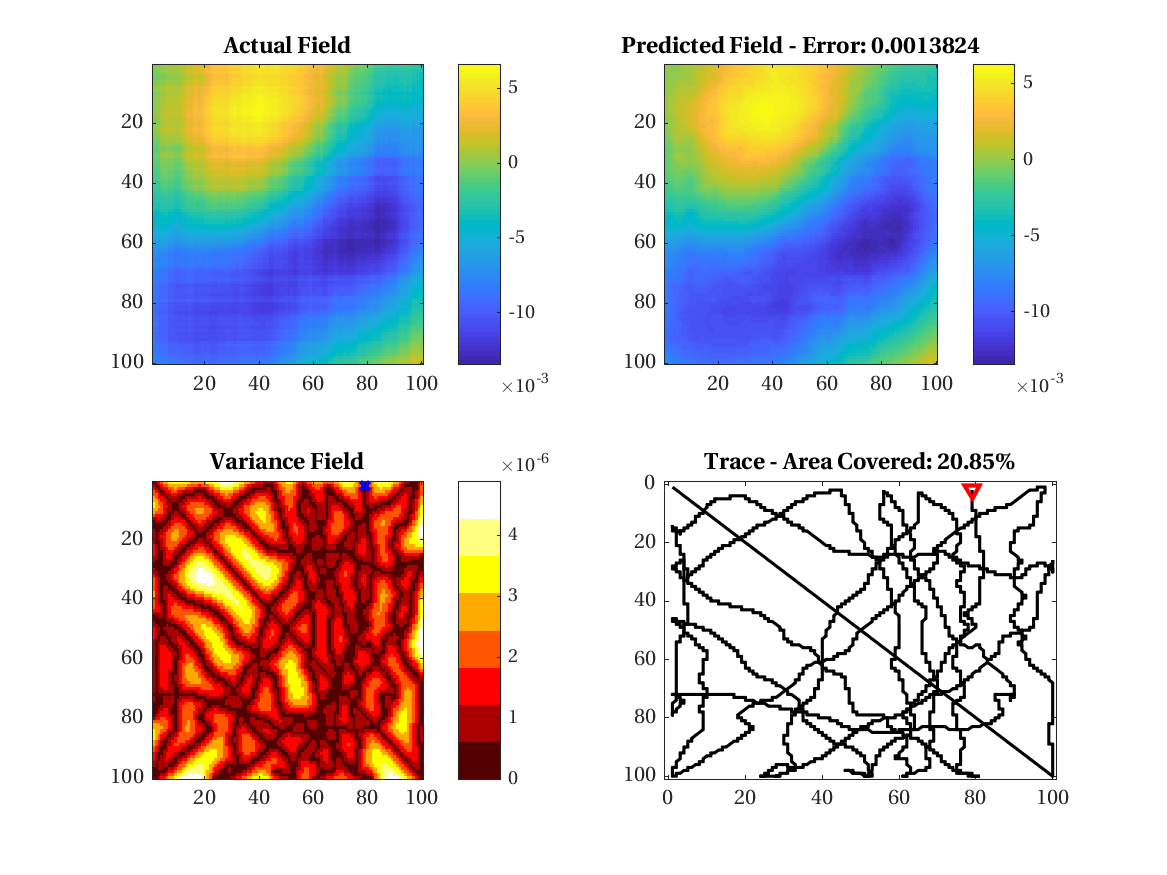
\includegraphics[width=\linewidth]{figures/hbresults/mc_20p_100x100_sf_25_seed_3.png}
        \captionsetup{skip=0.10\baselineskip,size=footnotesize}
        \caption{Monte Carlo Path Planner}
    \end{subfigure}%
    ~ 
    \begin{subfigure}[t]{0.5\textwidth}
        \centering
        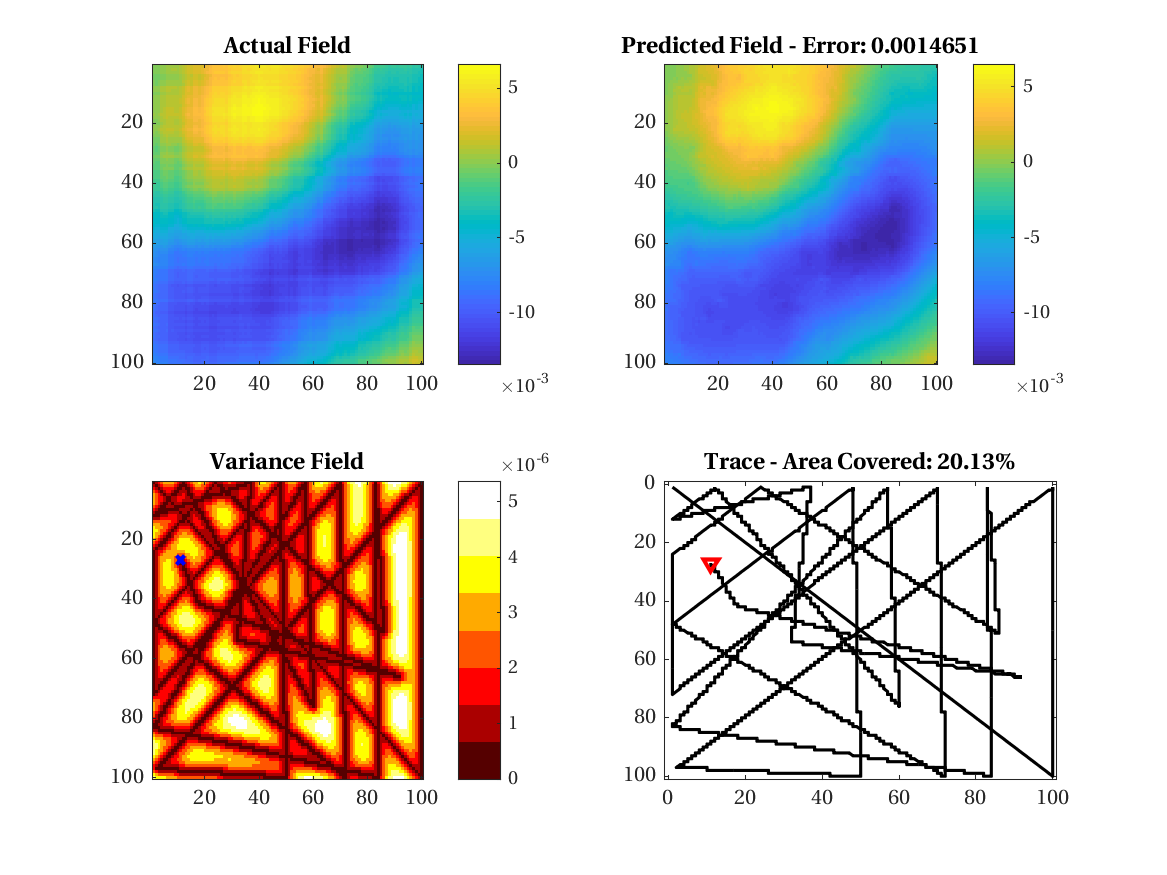
\includegraphics[width=\linewidth]{figures/hbresults/nhv_20p_100x100_sf_25_seed_3.png}
        \captionsetup{skip=0.10\baselineskip,size=footnotesize}
        \caption{Next Highest Variance Path Planner}
    \end{subfigure}%
    \\
    \begin{subfigure}[t]{0.5\textwidth}
        \centering
        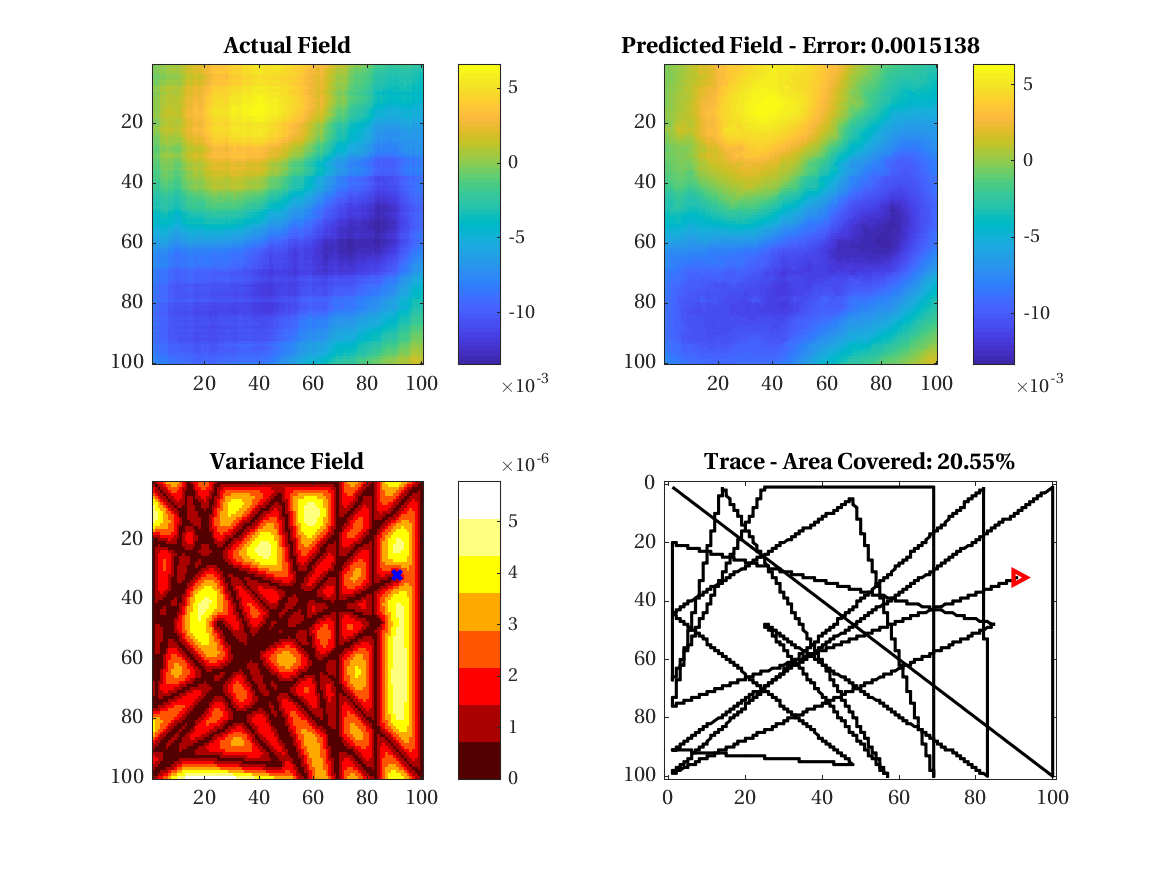
\includegraphics[width=\linewidth]{figures/hbresults/nnhv_20p_100x100_sf_25_seed_3.png}
        \captionsetup{skip=0.10\baselineskip,size=footnotesize}
        \caption{$N$ Next Highest Variance Path Planner}
    \end{subfigure}%
    ~
    \begin{subfigure}[t]{0.5\textwidth}
        \centering
        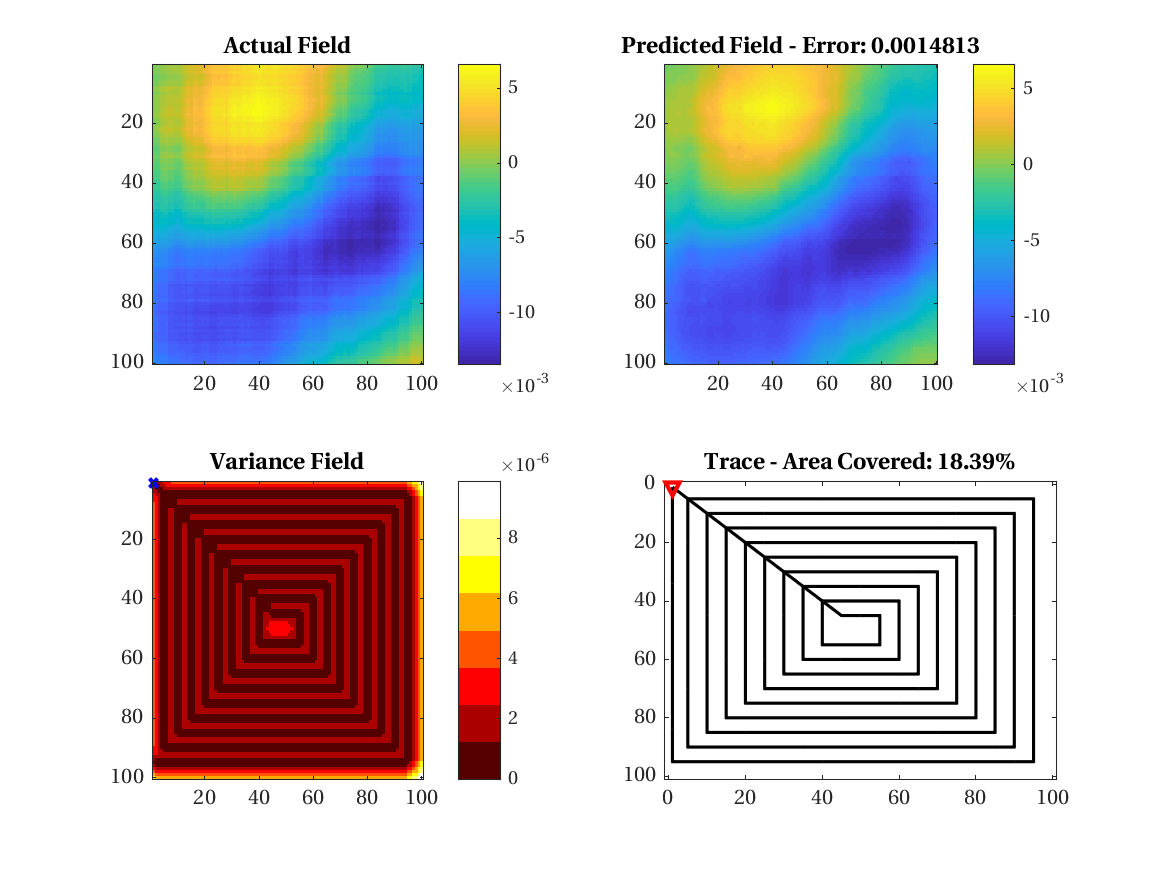
\includegraphics[width=\linewidth]{figures/hbresults/zz_20p_100x100_sf_25_seed_3.png}
        \captionsetup{skip=0.10\baselineskip,size=footnotesize}
        \caption{Zig-Zag Method}
    \end{subfigure}%
    \captionsetup{skip=0.20\baselineskip}
    \caption{Simulation output for a $20\%$ maximum area scan on a field of size $100 \times 100$, $\sigma_{field} = 25$, random seed: 3.}
    \label{fig:sim_sigma25_p20_s3}
\end{figure}

\FloatBarrier
\clearpage
\subsection{$30\%$ Maximum Field Scan}
\begin{figure}[htb!]
    \centering
    \begin{subfigure}[t]{0.65\textwidth}
        \centering
        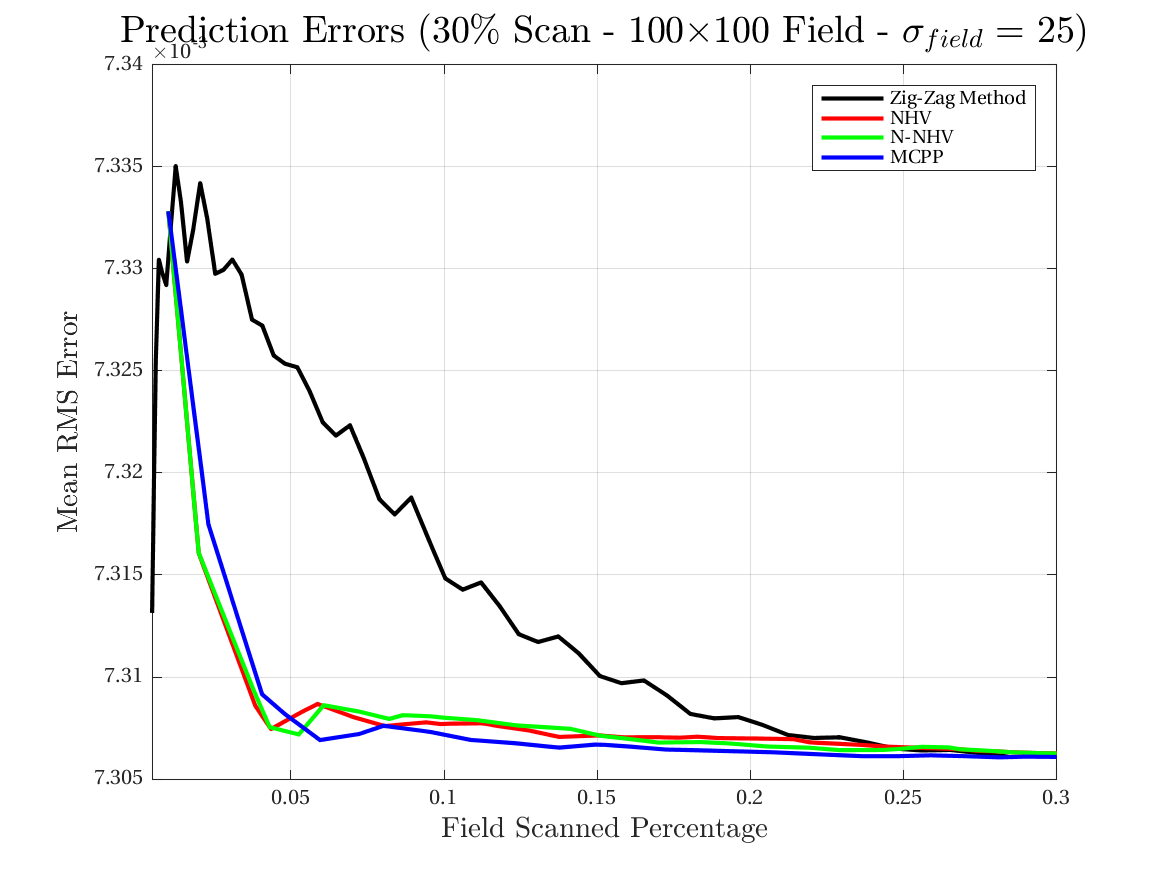
\includegraphics[width=\linewidth]{figures/hbresults/pred_errs_30p_100x100_sf_25_seed_3.png}
        \captionsetup{skip=0.20\baselineskip,size=footnotesize}
        \caption{Prediction errors (erf$(Z,\hat{Z})$).}
        \label{fig:prederrs_sigma25_p30_s3}
    \end{subfigure}%
    \\
    \begin{subfigure}[t]{0.65\textwidth}
        \centering
        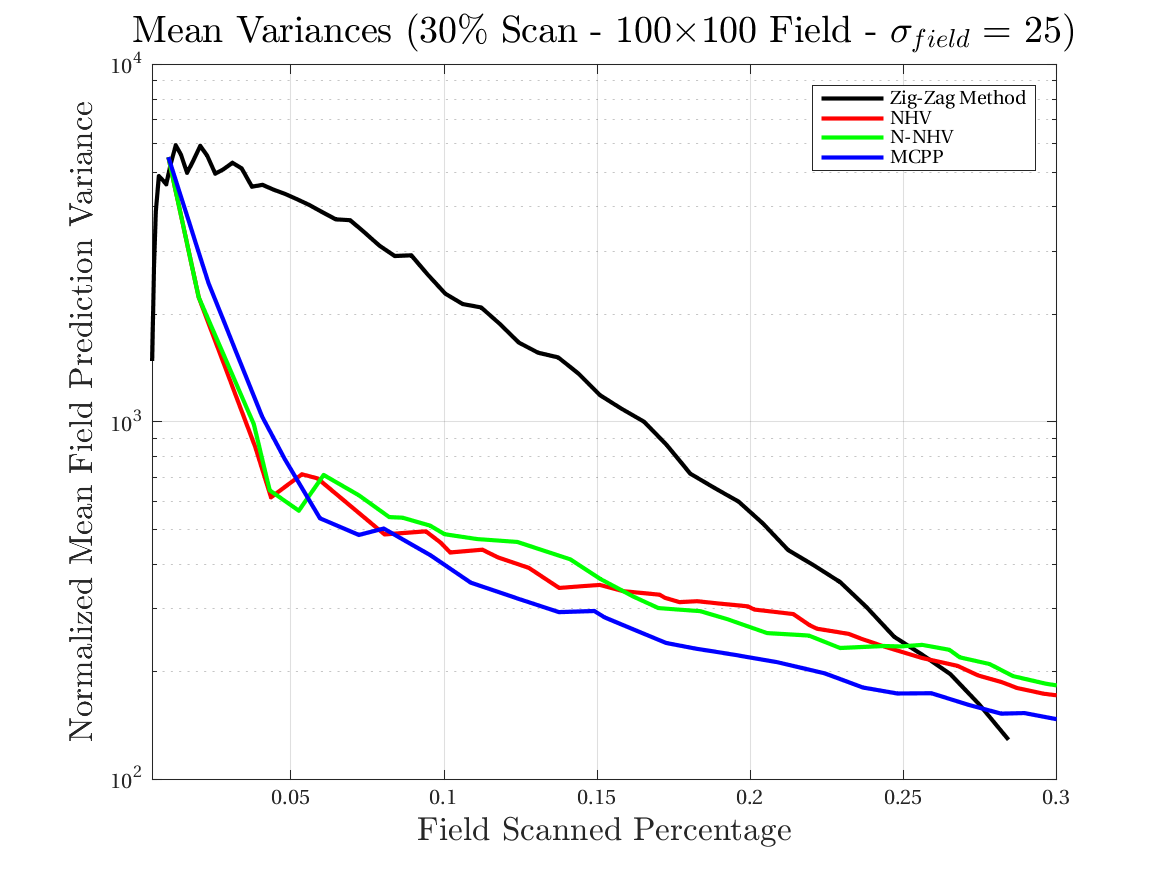
\includegraphics[width=\linewidth]{figures/hbresults/vars_30p_100x100_sf_25_seed_3.png}
        \captionsetup{skip=0.20\baselineskip,size=footnotesize}
        \caption{Semi-logarithmic prediction variances normalized to an a priori mean variance for the field.}
        \label{fig:prederrs_sigma25_p30_s3}
    \end{subfigure}
    \captionsetup{skip=0.20\baselineskip}
    \caption{A $30\%$ maximum area scan on a field of size $100 \times 100$, $\sigma_{field} = 25$, random seed: 3.}
    \label{fig:sigma25_p30_s3}
\end{figure}

\begin{figure}[htb!]
    \centering
    \begin{subfigure}[t]{0.5\textwidth}
        \centering
        \includegraphics[width=\linewidth]{figures/hbresults/mc_30p_100x100_sf_25_seed_3.png}
        \captionsetup{skip=0.10\baselineskip,size=footnotesize}
        \caption{Monte Carlo Path Planner}
    \end{subfigure}%
    ~ 
    \begin{subfigure}[t]{0.5\textwidth}
        \centering
        \includegraphics[width=\linewidth]{figures/hbresults/nhv_30p_100x100_sf_25_seed_3.png}
        \captionsetup{skip=0.10\baselineskip,size=footnotesize}
        \caption{Next Highest Variance Path Planner}
    \end{subfigure}%
    \\
    \begin{subfigure}[t]{0.5\textwidth}
        \centering
        \includegraphics[width=\linewidth]{figures/hbresults/nnhv_30p_100x100_sf_25_seed_3.png}
        \captionsetup{skip=0.10\baselineskip,size=footnotesize}
        \caption{$N$ Next Highest Variance Path Planner}
    \end{subfigure}%
    ~
    \begin{subfigure}[t]{0.5\textwidth}
        \centering
        \includegraphics[width=\linewidth]{figures/hbresults/zz_30p_100x100_sf_25_seed_3.png}
        \captionsetup{skip=0.10\baselineskip,size=footnotesize}
        \caption{Zig-Zag Method}
    \end{subfigure}%
    \captionsetup{skip=0.20\baselineskip}
    \caption{Simulation output for a $30\%$ maximum area scan on a field of size $100 \times 100$, $\sigma_{field} = 25$, random seed: 3.}
    \label{fig:sim_sigma25_p30_s3}
\end{figure}

%% LOW AC
\section{Low Spatial Autocorrelation Results}
The methods will be compared on target fields generated with a low autocorrelation factor ($\sigma_{field}=1$).

\clearpage
\subsection{$10\%$ Maximum Field Scan}
\begin{figure}[htb!]
    \centering
    \begin{subfigure}[t]{0.65\textwidth}
        \centering
        \includegraphics[width=\linewidth]{figures/hbresults/pred_errs_10p_100x100_sf_1_seed_3.png}
        \captionsetup{skip=0.20\baselineskip,size=footnotesize}
        \caption{Prediction errors (erf$(Z,\hat{Z})$).}
        \label{fig:prederrs_sigma1_p10_s3}
    \end{subfigure}%
    \\
    \begin{subfigure}[t]{0.65\textwidth}
        \centering
        \includegraphics[width=\linewidth]{figures/hbresults/vars_10p_100x100_sf_1_seed_3.png}
        \captionsetup{skip=0.20\baselineskip,size=footnotesize}
        \caption{Semi-logarithmic prediction variances normalized to an a priori mean variance for the field.}
        \label{fig:prederrs_sigma1_p10_s3}
    \end{subfigure}
    \captionsetup{skip=0.20\baselineskip}
    \caption{A $10\%$ maximum area scan on a field of size $100 \times 100$, $\sigma_{field} = 1$, random seed: 3.}
    \label{fig:sigma1_p10_s3}
\end{figure}

\begin{figure}[htb!]
    \centering
    \begin{subfigure}[t]{0.5\textwidth}
        \centering
        \includegraphics[width=\linewidth]{figures/hbresults/mc_10p_100x100_sf_1_seed_3.png}
        \captionsetup{skip=0.10\baselineskip,size=footnotesize}
        \caption{Monte Carlo Path Planner}
    \end{subfigure}%
    ~ 
    \begin{subfigure}[t]{0.5\textwidth}
        \centering
        \includegraphics[width=\linewidth]{figures/hbresults/nhv_10p_100x100_sf_1_seed_3.png}
        \captionsetup{skip=0.10\baselineskip,size=footnotesize}
        \caption{Next Highest Variance Path Planner}
    \end{subfigure}%
    \\
    \begin{subfigure}[t]{0.5\textwidth}
        \centering
        \includegraphics[width=\linewidth]{figures/hbresults/nnhv_10p_100x100_sf_1_seed_3.png}
        \captionsetup{skip=0.10\baselineskip,size=footnotesize}
        \caption{$N$ Next Highest Variance Path Planner}
    \end{subfigure}%
    ~
    \begin{subfigure}[t]{0.5\textwidth}
        \centering
        \includegraphics[width=\linewidth]{figures/hbresults/zz_10p_100x100_sf_1_seed_3.png}
        \captionsetup{skip=0.10\baselineskip,size=footnotesize}
        \caption{Zig-Zag Method}
    \end{subfigure}%
    \captionsetup{skip=0.20\baselineskip}
    \caption{Simulation output for a $10\%$ maximum area scan on a field of size $100 \times 100$, $\sigma_{field} = 1$, random seed: 3.}
    \label{fig:sim_sigma1_p10_s3}
\end{figure}

\FloatBarrier
\clearpage
\subsection{$20\%$ Maximum Field Scan}
\begin{figure}[htb!]
    \centering
    \begin{subfigure}[t]{0.65\textwidth}
        \centering
        \includegraphics[width=\linewidth]{figures/hbresults/pred_errs_20p_100x100_sf_1_seed_3.png}
        \captionsetup{skip=0.20\baselineskip,size=footnotesize}
        \caption{Prediction errors (erf$(Z,\hat{Z})$).}
        \label{fig:prederrs_sigma1_p20_s3}
    \end{subfigure}%
    \\
    \begin{subfigure}[t]{0.65\textwidth}
        \centering
        \includegraphics[width=\linewidth]{figures/hbresults/vars_20p_100x100_sf_1_seed_3.png}
        \captionsetup{skip=0.20\baselineskip,size=footnotesize}
        \caption{Semi-logarithmic prediction variances normalized to an a priori mean variance for the field.}
        \label{fig:prederrs_sigma1_p20_s3}
    \end{subfigure}
    \captionsetup{skip=0.20\baselineskip}
    \caption{A $20\%$ maximum area scan on a field of size $100 \times 100$, $\sigma_{field} = 1$, random seed: 3.}
    \label{fig:sigma1_p20_s3}
\end{figure}

\begin{figure}[htb!]
    \centering
    \begin{subfigure}[t]{0.5\textwidth}
        \centering
        \includegraphics[width=\linewidth]{figures/hbresults/mc_20p_100x100_sf_1_seed_3.png}
        \captionsetup{skip=0.10\baselineskip,size=footnotesize}
        \caption{Monte Carlo Path Planner}
    \end{subfigure}%
    ~ 
    \begin{subfigure}[t]{0.5\textwidth}
        \centering
        \includegraphics[width=\linewidth]{figures/hbresults/nhv_20p_100x100_sf_1_seed_3.png}
        \captionsetup{skip=0.10\baselineskip,size=footnotesize}
        \caption{Next Highest Variance Path Planner}
    \end{subfigure}%
    \\
    \begin{subfigure}[t]{0.5\textwidth}
        \centering
        \includegraphics[width=\linewidth]{figures/hbresults/nnhv_20p_100x100_sf_1_seed_3.png}
        \captionsetup{skip=0.10\baselineskip,size=footnotesize}
        \caption{$N$ Next Highest Variance Path Planner}
    \end{subfigure}%
    ~
    \begin{subfigure}[t]{0.5\textwidth}
        \centering
        \includegraphics[width=\linewidth]{figures/hbresults/zz_20p_100x100_sf_1_seed_3.png}
        \captionsetup{skip=0.10\baselineskip,size=footnotesize}
        \caption{Zig-Zag Method}
    \end{subfigure}%
    \captionsetup{skip=0.20\baselineskip}
    \caption{Simulation output for a $20\%$ maximum area scan on a field of size $100 \times 100$, $\sigma_{field} = 1$, random seed: 3.}
    \label{fig:sim_sigma1_p20_s3}
\end{figure}

\FloatBarrier
\clearpage
\subsection{$30\%$ Maximum Field Scan}
\begin{figure}[htb!]
    \centering
    \begin{subfigure}[t]{0.65\textwidth}
        \centering
        \includegraphics[width=\linewidth]{figures/hbresults/pred_errs_30p_100x100_sf_1_seed_3.png}
        \captionsetup{skip=0.20\baselineskip,size=footnotesize}
        \caption{Prediction errors (erf$(Z,\hat{Z})$).}
        \label{fig:prederrs_sigma1_p30_s3}
    \end{subfigure}%
    \\
    \begin{subfigure}[t]{0.65\textwidth}
        \centering
        \includegraphics[width=\linewidth]{figures/hbresults/vars_30p_100x100_sf_1_seed_3.png}
        \captionsetup{skip=0.20\baselineskip,size=footnotesize}
        \caption{Semi-logarithmic prediction variances normalized to an a priori mean variance for the field.}
        \label{fig:prederrs_sigma1_p30_s3}
    \end{subfigure}
    \captionsetup{skip=0.20\baselineskip}
    \caption{A $30\%$ maximum area scan on a field of size $100 \times 100$, $\sigma_{field} = 1$, random seed: 3.}
    \label{fig:sigma1_p30_s3}
\end{figure}

\begin{figure}[htb!]
    \centering
    \begin{subfigure}[t]{0.5\textwidth}
        \centering
        \includegraphics[width=\linewidth]{figures/hbresults/mc_30p_100x100_sf_1_seed_3.png}
        \captionsetup{skip=0.10\baselineskip,size=footnotesize}
        \caption{Monte Carlo Path Planner}
    \end{subfigure}%
    ~ 
    \begin{subfigure}[t]{0.5\textwidth}
        \centering
        \includegraphics[width=\linewidth]{figures/hbresults/nhv_30p_100x100_sf_1_seed_3.png}
        \captionsetup{skip=0.10\baselineskip,size=footnotesize}
        \caption{Next Highest Variance Path Planner}
    \end{subfigure}%
    \\
    \begin{subfigure}[t]{0.5\textwidth}
        \centering
        \includegraphics[width=\linewidth]{figures/hbresults/nnhv_30p_100x100_sf_1_seed_3.png}
        \captionsetup{skip=0.10\baselineskip,size=footnotesize}
        \caption{$N$ Next Highest Variance Path Planner}
    \end{subfigure}%
    ~
    \begin{subfigure}[t]{0.5\textwidth}
        \centering
        \includegraphics[width=\linewidth]{figures/hbresults/zz_30p_100x100_sf_1_seed_3.png}
        \captionsetup{skip=0.10\baselineskip,size=footnotesize}
        \caption{Zig-Zag Method}
    \end{subfigure}%
    \captionsetup{skip=0.20\baselineskip}
    \caption{Simulation output for a $30\%$ maximum area scan on a field of size $100 \times 100$, $\sigma_{field} = 1$, random seed: 3.}
    \label{fig:sim_sigma1_p30_s3}
\end{figure}